%% 
%% Copyright 2007, 2008, 2009 Elsevier Ltd
%% 
%% This file is part of the 'Elsarticle Bundle'.
%% ---------------------------------------------
%% 
%% It may be distributed under the conditions of the LaTeX Project Public
%% License, either version 1.2 of this license or (at your option) any
%% later version.  The latest version of this license is in
%%    http://www.latex-project.org/lppl.txt
%% and version 1.2 or later is part of all distributions of LaTeX
%% version 1999/12/01 or later.
%% 
%% The list of all files belonging to the 'Elsarticle Bundle' is
%% given in the file `manifest.txt'.
%% 

%% Template article for Elsevier's document class `elsarticle'
%% with numbered style bibliographic references
%% SP 2008/03/01

\documentclass[preprint,12pt]{elsarticle}
% -----PACKAGES
%\usepackage[shortend,titlenumbered]{algorithm2e}
%\usepackage{algorithmic}
%\usepackage[plain]{algorithm}
\usepackage{multicol}
\usepackage{color}
\usepackage{multirow}
\usepackage{fancybox}
%\usepackage{index}
\usepackage{varioref}
\usepackage{psfrag}
\usepackage{epsfig}
\usepackage{boxedminipage}
\usepackage{graphicx}
\usepackage{rotating}
\usepackage{amsmath}
\usepackage{amssymb}
%\usepackage{amsfont}
\usepackage{latexsym}
\usepackage{alltt}
%\usepackage[small,bf]{caption}
\usepackage{url}
%\usepackage{citesort}
%\usepackage{crop}
\usepackage{array}
\usepackage{subfigure}
\usepackage{dcolumn}

% -----SETLENGTH
%\setlength{\captionmargin}{20pt} 

% -----NEWCOMMANDS
\newcommand{\nc}{\newcommand}
\nc{\mathsm}[1]{\text{\small{$#1$}}}
\nc{\ubar}[1]{\underset{-}{#1}}
\nc{\optype}{\textrm}
\nc{\EQ}[1]{(\ref{eq:#1})}
\nc{\TAB}[1]{\ref{tab:#1}}
\nc{\FIG}[1]{\ref{fig:#1}}
\nc{\SEC}[1]{\ref{sec:#1}}
\nc{\ALG}[1]{\ref{alg:#1}}
\nc{\CHAP}[1]{\ref{chap:#1}}
\nc{\mtrx}[1]{\boldsymbol{\mathbf{#1}}}
\nc{\vctr}[1]{\boldsymbol{\mathbf{#1}}}
\nc{\grad}{\mbox{\boldmath$\nabla$}}
\nc{\gradient}{\textsl{grad}\,}
\nc{\hessian}{\textsl{grad\,}^2}
\nc{\ii}{\iota}
\nc{\dd}{d}
\nc{\ee}{\mathrm{e}}
\nc{\pdiv}[2]{\partial{#1}/\partial{#2}}
\nc{\dpdiv}[2]{\displaystyle{\frac{\partial{#1}}{\partial{#2}}}}
\nc{\ddiv}[2]{\displaystyle{\frac{\dd{#1}}{\dd{#2}}}}
\nc{\inpr}{\hspace{-1pt}\cdot\hspace{-1pt}}
\nc{\IR}{\mathbb{R}}
\nc{\IN}{\mathbb{N}}
\nc{\IZ}{\mathbb{Z}}
\nc{\IC}{\mathbb{C}}
\nc{\half}{\frac{1}{2}}
\nc{\shalf}{\scriptstyle{\half}} 
\nc{\ds}[1]{\displaystyle{#1}}
\nc{\ts}[1]{\textstyle{#1}}
\nc{\sign}{\optype{sign}}
\nc{\spr}{\optype{spr}}
\nc{\dist}{\optype{dist}}
\nc{\rank}{\optype{rank}}
\nc{\codim}{\optype{codim}}
\nc{\supp}{\optype{supp}}
\nc{\diag}{\optype{diag}}
\nc{\meas}{\optype{meas}}
\nc{\cond}{\optype{cond}}
\nc{\kernel}{\optype{kernel}}
\nc{\spa}{\optype{span}}
\nc{\order}{\mathcal{O}}
\nc{\Fr}{\mathrm{Fr}}
\nc{\Rey}{\mathrm{Re}}
\nc{\Ord}{O}
\nc{\ord}{o}
\nc{\st}{\:{:}\:}
\nc{\closure}[1]{\overline{#1}}
\nc{\emin}[1]{\emph{#1}\index{#1}\/}
\nc{\rmin}[1]{#1\index{{}@{#1}}}
\nc{\Laplace}{\Delta}
\nc{\ie}{i.e.}
\nc{\eg}{e.g.}
%\nc{\union}{\cup}
\nc{\Union}{\bigcup}
\nc{\lf}[1]{\mathsf{#1}}
\nc{\dbar}[1]{\bar{\bar{#1}}}
\nc{\ul}[1]{\underline{#1}}
\nc{\hpt}{\hspace{0.5pt}}
\nc{\E}[1]{\times{}10^{#1}}
\nc{\inp}[2]{\langle{#1},{#2}\rangle}
\nc{\tmpcommand}{}

% -----RENEWCOMMANDS
\renewcommand{\baselinestretch}{1}
\renewcommand{\exp}{\optype{exp}\,}
\renewcommand{\cosh}{\optype{cosh}\,}
\renewcommand{\tanh}{\optype{tanh}\,}
\renewcommand{\sinh}{\optype{sinh}\,}
\renewcommand{\div}[1]{\optype{div}\,{#1}}
\renewcommand{\half}{\mbox{$\frac{1}{2}$}}
%\renewcommand{\descriptionlabel}[1]{\hspace{\labelsep}\emph{#1}}

% -----ETC
\raggedbottom


\DeclareMathOperator{\curl}{\bf curl}
\DeclareMathOperator{\rot}{\rm curl}
\DeclareMathOperator{\divv}{\rm div}
\newcommand{\tro}{\gamma_0}
\newcommand{\trt}{\gamma_{\sft}}
\newcommand{\trn}{\gamma_{\sfn}}

\newcommand{\PT}{{\partial T}}
\newcommand{\bbN}{{\mathbb{N}}}
\newcommand{\bbP}{{\mathbb{P}}}

\newcommand{\scC}{{\mathscr{C}}}
\newcommand{\caD}{{\mathcal{D}}}
\newcommand{\caL}{{\mathcal{L}}}

\newcommand{\sfe}{{\mathsf{e}}}
\newcommand{\sff}{{\mathsf{f}}}
\newcommand{\sft}{{\boldsymbol{\mathsf{t}}}}
\newcommand{\sfn}{{\boldsymbol{\mathsf{n}}}}

%   Common caligraphic abbrevs
\newcommand{\BB}{\mathcal{B}}
\newcommand{\CC}{\mathcal{C}}
\newcommand{\DD}{\mathcal{D}}
\newcommand{\EE}{\mathcal{E}}
\newcommand{\FF}{\mathcal{F}}
\newcommand{\GG}{\mathcal{G}}
\newcommand{\II}{\mathcal{I}}
\newcommand{\JJ}{\mathcal{J}}
\newcommand{\KK}{\mathcal{K}}
\newcommand{\LL}{\mathcal{L}}
\newcommand{\OO}{\mathcal{O}}
\newcommand{\QQ}{\mathcal{Q}}
\newcommand{\RR}{\mathcal{R}}
\newcommand{\TT}{\mathcal{T}}


 %% JAY'S PREAMBLE
 %%========================

%   Math symbol definitions
\def\d{\partial}
%\newsymbol\lee 132E
\newcommand{\union}{\mathop{\bigcup}}
\newcommand{\intersect}{\mathop{\bigcap}}
\newcommand{\binomial}[2]{\ensuremath{
		\begin{pmatrix}{#1}\\{#2}\end{pmatrix}}}
\newcommand{\smallbinomial}[2]{\ensuremath{
		(\begin{smallmatrix}{#1}\\{#2}\end{smallmatrix})}}
\newcommand{\tang}[1]{\ensuremath{{#1}_{\intercal}}} % can use \top
						     % also
\newcommand{\hypergeom}[2]{\ensuremath{\sideset{_{#1}}{_{#2}}{\mathop{F}}}}
%   Difficult names
\newcommand{\Babuska}{Babu{\v{s}}ka}       % Remember: Usage is \Babuska\
\newcommand{\Cea}{C{\'e}a}                 % with trailing `\' to give space
\newcommand{\Poincare}{Poincar{\'{e}}}     % when needed, but when ending
\newcommand{\Nedelec}{N{\'{e}}d{\'{e}}lec} % sentence use \Babuska.
\newcommand{\Frechet}{Fr{\'{e}}chet}
\newcommand{\Muller}{M{\"u}ller}
\newcommand{\LHospital}{L'H{\^{o}}spital}
%   Bold and beautiful
\newcommand{\ba}{{\boldsymbol{a}}}
\newcommand{\bA}{\boldsymbol{A}}
\newcommand{\balpha}{{\boldsymbol{\alpha}}}
\newcommand{\bB}{{\boldsymbol{B}}}
\newcommand{\bb}{{\boldsymbol{b}}}
\newcommand{\bbeta}{{\boldsymbol{\beta}}}
\newcommand{\etab}{{\boldsymbol{\eta}}}
\newcommand{\bC}{{\boldsymbol{C}}}
\newcommand{\bc}{{\boldsymbol{c}}}
\newcommand{\bD}{{\boldsymbol{D}}}
\newcommand{\bd}{{\boldsymbol{d}}}
\newcommand{\db}{{\boldsymbol{\d}}}
\newcommand{\bdelta}{{\boldsymbol{\delta}}}
\newcommand{\bDelta}{{\boldsymbol{\Delta}}}
\newcommand{\beps}{{\boldsymbol{\varepsilon}}}
\newcommand{\be}{{\boldsymbol{e}}}
\newcommand{\bg}{{\boldsymbol{g}}}
\newcommand{\bm}{{\boldsymbol{m}}}
\newcommand{\bn}{{\boldsymbol{n}}}
\newcommand{\bN}{{\boldsymbol{N}}}
\newcommand{\bp}{{\boldsymbol{p}}}
\newcommand{\bpsi}{{\boldsymbol{\psi}}}
\newcommand{\bq}{{\boldsymbol{q}}}
\newcommand{\bxi}{{\boldsymbol{\xi}}}
\newcommand{\bE}{{\boldsymbol{E}}}
\newcommand{\bF}{{\boldsymbol{F}}}
\newcommand{\bh}{{\boldsymbol{h}}}
\newcommand{\bH}{{\boldsymbol{H}}}
\newcommand{\bI}{{\boldsymbol{I}}}
\newcommand{\bj}{{\boldsymbol{j}}}
\newcommand{\bJ}{{\boldsymbol{J}}}
\newcommand{\bK}{{\boldsymbol{K}}}
\newcommand{\bk}{{\boldsymbol{k}}}
\newcommand{\bll}{{\boldsymbol{\ell}}}
\newcommand{\bL}{{\boldsymbol{L}}}
\newcommand{\blambda}{{\boldsymbol{\lambda}}}
\newcommand{\bmu}{{\boldsymbol{\mu}}}
\newcommand{\bM}{{\boldsymbol{M}}}
\newcommand{\bomega}{{\boldsymbol{\omega}}}
\newcommand{\bP}{{\boldsymbol{P}}}
\newcommand{\bphi}{{\boldsymbol{\phi}}}
\newcommand{\bQ}{{\boldsymbol{Q}}}
\newcommand{\bG}{{\boldsymbol{G}}}
\newcommand{\bu}{{\boldsymbol{u}}}
\newcommand{\bU}{{\boldsymbol{U}}}
\newcommand{\bV}{{\boldsymbol{V}}}
\newcommand{\bX}{{\boldsymbol{X}}}
\newcommand{\bv}{{\boldsymbol{v}}}
\newcommand{\bw}{{\boldsymbol{w}}}
\newcommand{\bW}{{\boldsymbol{W}}}
\newcommand{\bR}{{\boldsymbol{R}}}
\newcommand{\br}{{\boldsymbol{r}}}
\newcommand{\bS}{{\boldsymbol{S}}}
\newcommand{\bT}{{\boldsymbol{T}}}
\newcommand{\btau}{{\boldsymbol{\tau}}}
\newcommand{\bt}{{\boldsymbol{t}}}
\newcommand{\bx}{{\boldsymbol{x}}}
\newcommand{\by}{{\boldsymbol{y}}}
\newcommand{\bz}{{\boldsymbol{z}}}
\newcommand{\bzero}{{\boldsymbol{0}}}
\newcommand{\bZ}{{\boldsymbol{Z}}}
%   Common scalar fields
\newcommand{\RRR}{\mathbb{R}}
\newcommand{\CCC}{\mathbb{C}}
\newcommand{\ZZZ}{\mathbb{Z}}
\newcommand{\NNN}{\mathbb{N}}
%   Differential operators
\newcommand{\dive}{\mathop\mathrm{div}}
%\newcommand{\grad}{\ensuremath{\mathop{{\bf{grad}}}}}
%\newcommand{\curl}{{\ensuremath\mathop{\mathbf{curl}\,}}}
\newcommand{\Curl}{ {\bf Curl}}
\newcommand{\dx}{\ensuremath{\mathrm{d}x}}
\newcommand{\dy}{\ensuremath{\mathrm{d}y}}
\newcommand{\dr}{\ensuremath{\mathrm{d}r}}
\newcommand{\dR}{\ensuremath{\mathrm{d}R}}
\newcommand{\drho}{\ensuremath{\mathrm{d}\rho}}
\newcommand{\dz}{\ensuremath{\mathrm{d}z}}
\newcommand{\dzeta}{\ensuremath{\mathrm{d}\zeta}}
%   Wordy math symbols
\newcommand{\card}{\ensuremath{\mathop\mathrm{card}}}
%\newcommand{\diag}{\ensuremath{\mathop\mathrm{diag}}}
\newcommand{\diam}{\ensuremath{\mathop\mathrm{diam}}}
%\newcommand{\dist}{\mathop\mathrm{dist}}
\newcommand{\Ker}{\mathop\mathrm{Ker}}
\newcommand{\Range}{\mathop\mathrm{Range}}
%\newcommand{\rank}{\mathop\mathrm{rank}}
%\newcommand{\meas}{\mathop\mathrm{meas}}
\newcommand{\Forall}{\quad\text{for all }}
%\newcommand{\supp}{\mathop\mathrm{supp}}
\newcommand{\Span}{\mathop\mathrm{Span}}
\newcommand{\Hdiv}[1]{\bH(\dive,#1)}
%\newcommand{\Hcurl}[1]{\bH(\curl,#1)}
%   Common caligraphic abbrevs
%\newcommand{\BB}{\mathcal{B}}
%\newcommand{\CC}{\mathcal{C}}
%\newcommand{\DD}{\mathcal{D}}
%\newcommand{\EE}{\mathcal{E}}
%\newcommand{\FF}{\mathcal{F}}
%\newcommand{\GG}{\mathcal{G}}
%\newcommand{\II}{\mathcal{I}}
%\newcommand{\JJ}{\mathcal{J}}
%\newcommand{\KK}{\mathcal{K}}
%\newcommand{\LL}{\mathcal{L}}
%\newcommand{\OO}{\mathcal{O}}
%\newcommand{\QQ}{\mathcal{Q}}
%\newcommand{\RR}{\mathcal{R}}
%\newcommand{\TT}{\mathcal{T}}
%   Variations on standard symbols
\newcommand{\veps}{\varepsilon}
\newcommand{\vlam}{\varLambda}
\newcommand{\vpi}{\varPi}
\newcommand{\vPi}{\boldsymbol{\varPi}}
\newcommand{\vsig}{\varSigma}
\newcommand{\vbt}{\boldsymbol{\varTheta}}
\newcommand{\vPsi}{\boldsymbol{\varPsi}}
%\newcommand{\ii}{\hat{\imath}}
%   Innerproducts, norms, etc
\newcommand{\ntrip}[1]{|\!|\!| {#1} |\!|\!|}
\newcommand{\ip}[1]{\langle {#1} \rangle}
%   Utilities
\newcommand{\blnk}{\underline{\hspace{3cm}}\;}
\newcommand{\marg}[1]{\marginpar{\tiny{\framebox{\parbox{1.7cm}{#1}}}}}
\newcommand{\degreeC}[1]{\ensuremath{{#1\,}^\circ\!\text{C}}}
                        % try also  \textcelsius of textcomp package
%   Trademarked names \texttrademark, \textregistered
\newcommand{\matlab}{MATLAB\textregistered\renewcommand{\matlab}{MATLAB}}
\newcommand{\femlab}{FEMLAB\textregistered\renewcommand{\femlab}{FEMLAB}}

%   Style preferences
\renewcommand{\thefootnote}{\fnsymbol{footnote}} % Use symbols instead of
						 % numbers for footnotes
						 

\newcommand{\Eg}{\EE^\mathrm{grad}}
\newcommand{\Ec}{\boldsymbol{\EE}^\mathrm{curl}}
\newcommand{\Ed}{\boldsymbol{\EE}^\mathrm{div}}


\newcommand{\bfdu}{\mbox{\boldmath $\delta u$}}
\newcommand{\bfdv}{\mbox{\boldmath $\delta v$}}
\newcommand{\du}{{\delta u}}
\newcommand{\dv}{{\delta v}}
\newcommand{\bfnabt}{\widetilde{\bfnab}}
\newcommand{\bfepst}{\widetilde{\bfeps}}

\graphicspath{{../Proposal/figs/}}

%% Use the option review to obtain double line spacing
%% \documentclass[authoryear,preprint,review,12pt]{elsarticle}

%% Use the options 1p,twocolumn; 3p; 3p,twocolumn; 5p; or 5p,twocolumn
%% for a journal layout:
%% \documentclass[final,1p,times]{elsarticle}
%% \documentclass[final,1p,times,twocolumn]{elsarticle}
%% \documentclass[final,3p,times]{elsarticle}
%% \documentclass[final,3p,times,twocolumn]{elsarticle}
%% \documentclass[final,5p,times]{elsarticle}
%% \documentclass[final,5p,times,twocolumn]{elsarticle}

%% For including figures, graphicx.sty has been loaded in
%% elsarticle.cls. If you prefer to use the old commands
%% please give \usepackage{epsfig}

%% The amssymb package provides various useful mathematical symbols
\usepackage{amssymb}
%% The amsthm package provides extended theorem environments
%% \usepackage{amsthm}

%% The lineno packages adds line numbers. Start line numbering with
%% \begin{linenumbers}, end it with \end{linenumbers}. Or switch it on
%% for the whole article with \linenumbers.
%% \usepackage{lineno}

\journal{Computers and Fluids}

\begin{document}

\begin{frontmatter}

%% Title, authors and addresses

%% use the tnoteref command within \title for footnotes;
%% use the tnotetext command for theassociated footnote;
%% use the fnref command within \author or \address for footnotes;
%% use the fntext command for theassociated footnote;
%% use the corref command within \author for corresponding author footnotes;
%% use the cortext command for theassociated footnote;
%% use the ead command for the email address,
%% and the form \ead[url] for the home page:
%% \title{Title\tnoteref{label1}}
%% \tnotetext[label1]{}
%% \author{Name\corref{cor1}\fnref{label2}}
%% \ead{email address}
%% \ead[url]{home page}
%% \fntext[label2]{}
%% \cortext[cor1]{}
%% \address{Address\fnref{label3}}
%% \fntext[label3]{}

\title{Space-Time DPG: Designing a Method for Massively Parallel CFD}

%% use optional labels to link authors explicitly to addresses:
%% \author[label1,label2]{}
%% \address[label1]{}
%% \address[label2]{}

\author[ices]{Truman E.~Ellis\corref{cor1}}
\ead{truman@ices.utexas.edu}
\author[ices]{Leszek F.~Demkowicz}
\author[anl]{Nathan V.~Roberts}
\author[rice]{\\Jesse L.~Chan}
\author[ices]{Robert D.~Moser}

\address[ices]{Institute for Computational Engineering and Sciences,
University of Texas at Austin
201 East 24th St, Stop C0200, Austin, TX 78703}
\address[anl]{Argonne Leadership Computing Facility,
Argonne National Laboratory
9700 South Cass Avenue Building 240, Argonne, IL 60439}
\address[rice]{Computational and Applied Mathematics,
Rice University
6100 Main MS-134, Houston, TX 77005}

\begin{abstract}
% The discontinuous Petrov-Galerkin method is a novel finite element framework with exceptional stability and adaptivity properties.
% Initial mesh design is a time consuming and expensive part of CFD simulations as a domain expert has to manually design the 
% mesh to achieve near resolution in all parts of the domain lest the numerical method become unstable.
% DPG in contrast does not have a pre-asymptotic regime, allowing simulations to start on the coarsest mesh that can adequately represent the domain geometry.
% \emph{A posteriori} error estimation and adaptivity can also be done very naturally as DPG comes with an error representation function 
% that indicates error in the energy norm.

% Automatic adaptivity and pre-asymptotic stability produce a powerful synergy when combined with high performance computing.
% Human intervention to correct or adapt a failed massively parallel simulation can be a costly endeavor, prompting the desire for a
% numerical technology that will automatically adapt to changing physical dynamics while avoiding ``crashing'' due to under-resolved meshes.
% An ideal parallel algorithm should be locally compute intensive while maintaining minimal memory requirements.
% These are all observed properties of the discontinuous Petrov-Galerkin finite element method.
% Locally computed \emph{optimal test functions} ensure stability on convection dominated flows as well as resolved viscous flow.
% Individual contributions from each element to the global stiffness matrix can be computed completely independently due to the discontinuous nature of DPG.
% Furthermore, static condensation allows the global solve to concern only the \emph{trace} degrees of freedom; 
% trace variables are defined on the mesh skeleton.  
% This allows significant reduction of the cost of the global solve.  
% The internal degrees of freedom can then be resolved using a fully parallel post-processing step.

% We recently began exploring the extension of these attractive DPG properties to space-time domains, allowing us to automate and localize temporal adaptivity
% in the same way that we already do with spatial adaptivity. Preliminary results have been generated with Camellia\cite{Roberts2011} for spatially 1D flows,
% and a rewrite of Camellia for higher dimensions is currently in progress.
\end{abstract}

\begin{keyword}
%% keywords here, in the form: keyword \sep keyword

%% PACS codes here, in the form: \PACS code \sep code

%% MSC codes here, in the form: \MSC code \sep code
%% or \MSC[2008] code \sep code (2000 is the default)
Discontinuous Petrov-Galerkin \sep
Finite Elements \sep
Space-Time \sep
Navier-Stokes
\end{keyword}

\end{frontmatter}

%% \linenumbers

%% main text
\section{Introduction}
Initial mesh design for computational fluid dynamics can be a time-consuming and expensive process. 
The stability properties and nonlinear convergence of most numerical methods rely on a minimum level of mesh resolution. 
This means that unless the initial computational mesh is fine enough, convergence can not be guaranteed. 
Any meshes below this minimum resolution level are termed to be in the ``pre-asymptotic regime.'' 
This condition implies that meshes need to in some way anticipate the solution before it is known. 
On top of the minimum requirement that the surface meshes must adequately represent the geometry of the problem under consideration, 
resolution requirements on the volume mesh make the CFD practitioners job significantly more time consuming. 
This is not to mention auxiliary requirements from turbulence models needed to accurately resolve boundary layers. 
Thus, mesh design and simulation become an iterative trial and error process.
A common process is for an engineer to study the problem at hand and attempt to predict regions that require extra resolution. 
Then they will spend hours coaxing the mesher to produce an adequate mesh before importing the mesh into the solver.
Too often, the solver will fail to converge on the given mesh due to some unforeseen mesh inadequacy on part of the solution domain.
The engineer then needs to descend back into the mesher to fix the problem elements.
This process is repeated until the solver is satisfied and convergence can be reached.
This iterative trial and error is undesirable while working on personal computers or modestly sized compute clusters, 
but becomes increasing costly as the problem is scaled up to the tens or hundreds of thousands of processors common in high performance computing environments.

In contrast to most other numerical methods, the discontinuous Petrov-Galerkin finite element method retains exceptional stability on extremely coarse meshes.
DPG is also inherently very adaptive.
It is possible to compute the residual error without knowledge of the exact solution, which can be used to robustly drive adaptivity.
This results in a very automated technology, as the user can initialize a computation on the coarsest mesh which adequately represents the geometry 
then step back and let the program solve and adapt iteratively until it resolves the solution features.

\section{Overview of DPG}
% The discontinuous Petrov-Galerkin finite element method with optimal test functions 
% was first proposed by Demkowicz and Gopalakrishnan in 2009\cite{DPG1, DPG2}.
For a full treatment of the various ideas in DPG, please see \cite{DPGOverview2}.
The basic ideas are fairly straight-forward; DPG minimizes the residual in a user defined energy norm.
Consider a variational problem: find $u\in U$ such that
\[
b(u,v)=l(v) \quad\forall v\in V
\]
with operator $B:U\rightarrow V'\quad$ ($V'$ is the dual space to $V$) defined by $b(u,v)=\LRa{Bu,v}_{V'\times V}$.
This gives the operator equation:
\[
Bu=l\in V'\,.
\]
We wish to minimize the residual $Bu-l$ in $V'$:
\[
u_h=\argmin_{w_h\in U_h}\frac{1}{2}\norm{Bu-l}^2_{V'}\,.
\]
This is a very natural mathematical framework based soundly in functional analysis, but it is not yet a practical method as the $V'$ norm is not
especially tractable to work with.
The insight is that since we are working with Hilbert spaces, we can use the Riesz representation theorem to find a complementary object 
in $V$ rather than $V'$. Let $R_V:V\ni v\rightarrow(v,\cdot)\in V'$ be the Riesz map. 
Then the inverse Riesz map (which is an isometry) lets us represent our residual in $V$:
\[
u_h=\argmin_{w_h\in U_h}\frac{1}{2}\norm{R_V^{-1}(Bu-l)}^2_{V}\,.
\]
Taking the G\^ateaux derivative to be zero in all directions $\delta u \in
U_h$ gives,
\[
\left(R_V^{-1}(Bu_h-l),R_V^{-1}B\delta u\right)_V = 0, \quad \forall \delta u \in U,
\]
which by definition of the Riesz map is equivalent to 
\begin{equation*}
\LRa{Bu_h-l,R_V^{-1}B\delta u_h}=0\quad\forall\delta u_h\in U_h\,,
\end{equation*}
with optimal test functions $v_{\delta u_h}\coloneqq R_V^{-1}B\delta u_h$ for each trial function $\delta u_h$.
This gives a simple bilinear form
\begin{equation*}
b(u_h,v_{\delta u_h})=l(v_{\delta u_h}),
\end{equation*}
with $v_{\delta u_h}\in V$ that solves the auxiliary problem
\begin{equation*}
\LRp{v_{\delta u_h},\delta v}_V=\LRa{R_Vv_{\delta u_h},\delta v}
=\LRa{B\delta u_h,\delta v}=b(\delta u_h,\delta v)\quad\forall\delta v\in V.
\end{equation*}
We might call this an \emph{optimal Petrov-Galerkin}.
We arrive at the same method by realizing the supremum in the inf-sup condition, motivating the \emph{optimal} nomenclature.
These optimal Petrov-Galerkin methods produce Hermitian, positive-definite stiffness matrices since
\[
b(u_h,\vdeltau)=(v_{u_h},\vdeltau)_V=\overline{(\vdeltau,v_{u_h})}=\overline{b(\delta u_h,v_{u_h})}\,.
\]
We can calculate the energy norm (defined by $\norm{u}_E:=\norm{Bu}_{V'}$) of the Galerkin error without knowing the exact solution by using the residual:
\[
\norm{u_h-u}_E=\norm{B(u_h-u)}_{V'}=\norm{Bu_h-l}_{V'}=\norm{R_V^{-1}(Bu_h-l)}_V\,,
\]
where we designate $R_V^{-1}(Bu_h-l)$ the \emph{error representation function}.
This has proven to be a very reliable \emph{a-posteriori} error estimator for driving adaptivity.

Babu\v{s}ka's theorem\cite{Babuska70} says that discrete stability and approximability imply convergence.
That is, if $M$ is the continuity constant for $b(u,v)$ which satisfies the discrete inf-sup condition with constant $\gamma_h$,
\[
\sup_{v_h\in V_h}\frac{|b(u,v)|}{\norm{v_h}_V}\geq\gamma_h\norm{u_h}_U\,,
\]
then the Galerkin error satisfies the bound
\[
\norm{u_h-u}_U\leq\frac{M}{\gamma_h}\inf_{w_h\in U_h}\norm{w_h-u}_U\,.
\]
Optimal test functions realize the supremum in the discrete discrete inf-sup condition such that $\gamma_h\geq\gamma$, 
the infinite-dimensional inf-sup constant.
If we then use the energy norm for $\norm{\cdot}_U$, then $M=\gamma=1$ and Babu\v{s}ka's estimate implies that
the optimal Petrov-Galerkin method is the most stable Petrov-Galerkin method possible.

There are still many features of the method that are left to be decided, for example the $U$ and $V$ spaces.
If $V$ is taken to be a continuous space, then the auxiliary problem becomes global in scope, something that we would like to avoid.
In order to ensure the auxiliary problem can be solved element-by-element, we take $V$ to be discontinuous between elements.
(Technically, $V$ should also be infinite dimensional, but we have found it to be sufficient to use an ``enriched'' space of higher
polynomial dimension than the trial space\cite{PracticalDPG}.)
The downside to using discontinuous test functions is that it introduces new interface unknowns.
When the equations are integrated by parts over each element, the jump in test functions introduces new unknowns on the mesh skeleton
that would have gone away with continuous test functions.
Moro \etal\cite{MoroNguyenPeraire11} handle the flux unknowns with a numerical flux in the hybridized DPG method, but the standard DPG method treats
these as new unknowns to be solved for.
We still haven't specified our trial space $U$, but the rule is that for every integration by parts, a new skeleton unknown is introduced.
Most DPG considerations break a second order PDE into a system of first order PDEs which introduces a trace unknown (from the constitutive law) 
and a flux unknown (from the conservation law), but Demkowicz and Gopalakrishnan also formulated a \emph{primal DPG} method for second order equations
that does not introduce a trace unknown.
The overall number of interface unknowns in the primal DPG method is the same, however, since the solution is required to be $H^1$ conforming 
and the trace unknowns are essentially hidden here.

The final unresolved choice is what norm to apply to the $V$ space.
This is one of the most important factors in designing a robust DPG method as this norm needs to be inverted to solve for the optimal test functions.
If the norm produces unresolved boundary layers in the auxiliary problem, then many of the attractive features of DPG may fall apart.
But elimination of boundary layers in the auxiliary solve is not the only requirement at play. 
This choice also controls what norm the residual is minimized in. 
Often we want this norm to be equivalent to the $L^2$ norm.
Fortunately, we have found that it is possible to design test norms such that the implied energy norm 
is provably robust and equivalent to $L^2$ for convection-diffusion which
serves as the most relevant model problem for our research.
Norms for Navier-Stokes are derived by analogy to the convection-diffusion norm.

% DPG has been successfully applied to a wide range of physical problems.
% Early work on the Poisson equation was published in \cite{DPGPoisson}.
% Demkowicz \etal\cite{DPGHelmholtz}, Gopalakrishnan \etal\cite{Gopalakrishnan2014}, and Zitelli \etal\cite{DPG4} 
% analyzed and solved the Helmholtz equation with DPG.
% DPG was applied to linear elasticity and plate problems in \cite{BramwellDPG}, \cite{NiemiBramwellDemkowicz10}, and \cite{BramwellDemkowiczQiu10}.
% A 2D Maxwell cloaking problem was solved wit DPG in \cite{DPGCloaking} 
% and a 3D DPG theory for Maxwell was developed by Wieners and Wohlmuth\cite{WohlmuthReport}.
% DPG has been applied to various fluid problems including convection-diffusion\cite{DPG3,DemkowiczHeuer,ChanHeuerThanhDemkowicz2012,Chan2013,EllisLC},
% Stokes\cite{DPGStokes,EllisLC}, Burgers' equation\cite{Chan2013dpg}, incompressible Navier-Stokes\cite{NateDissertation}, 
% and compressible Navier-Stokes\cite{JesseDissertation}.


%   /$$   /$$ /$$$$$$$   /$$$$$$ 
%  | $$  | $$| $$__  $$ /$$__  $$
%  | $$  | $$| $$  \ $$| $$  \__/
%  | $$$$$$$$| $$$$$$$/| $$      
%  | $$__  $$| $$____/ | $$      
%  | $$  | $$| $$      | $$    $$
%  | $$  | $$| $$      |  $$$$$$/
%  |__/  |__/|__/       \______/ 
%                                
%                                
%   
\subsection{DPG for High Performance Computing}
Many of the features inherent in the DPG method appear promising in the context of high performance computing.
Our goal is to design a method that eliminates human intervention as much as possible.
The superior stability of the method promises to prevent a simulation from crashing which could eliminate expensive restarts on large systems.
Preliminary studies on convection-diffusion indicate exceptional robustness of the method in terms of diminishing viscosity, 
promising successful application to a large class of flow problems.
The adaptivity lent by the \emph{error representation function} provides a reliable and automated way to start from a coarse mesh and only refine
toward solution features in need. 
This uses compute resources much more efficiently than uniform refinements, allowing larger simulations with fewer resources.
These features combine to produce a high degree of automaticity.
Ultimately, it is desirable that an engineer could produce a rough mesh that just captures the geometry of the problem and
start a DPG simulation that automatically picks up solution features without the user needing to jump back in and fix things.

DPG is very compute intensive compared to the associated communication and memory costs.
Most of the work is spent in embarrassingly parallel local solves for the optimal test functions and local stiffness matrix assembly.
Additionally, the stability properties of DPG make high order solves a triviality, and in general, 
high order methods tend to have a more attractive compute/memory/communication profile than low order methods.
In our codes, we use QR factorization for the optimal test function solves, but this factorization is recyclable as we essentially have many right hand sides.
The division of degrees of freedom into internal vs skeleton unknowns produces a global system which can be statically condensed into 
a solve purely in terms of the skeleton degrees of freedom.
In addition to significantly cutting down on the size of the global solve, 
this produces a embarrassingly parallel post-processing solve for the internal degrees of freedom.
This property was one of the motivations behind the development of the hybridized discontinuous Galerkin\cite{HDG} method.
No matter what system of equations is being considered, DPG always produces a Hermitian (symmetric if real) 
positive definite stiffness matrix for the global solve.
This property has not really been leveraged in our simulations so far, since we have focused on direct rather than iterative solvers, but we
anticipate it might be an attractive feature in the future.
As compute resources scale up, many more HPC simulations are increasingly becoming coupled in multiphysics simulations.
Since the only requirement for a well-defined discrete DPG method is a well-defined continuous problem, it is certainly possible that each different part of the multiphysics simulation could be discretized with DPG -- no need to develop many different methods for each part of the simulation.
Already DPG has been successfully applied to domains as disparate as solid mechanics\cite{BramwellDPG}, Helmholtz\cite{DPGHelmholtz}, 
Navier-Stokes\cite{NateDissertation,JesseDissertation}, and Maxwell's equations\cite{PracticalDPG}.

%    /$$$$$$                                                  /$$$$$$$$ /$$                        
%   /$$__  $$                                                |__  $$__/|__/                        
%  | $$  \__/  /$$$$$$   /$$$$$$   /$$$$$$$  /$$$$$$            | $$    /$$ /$$$$$$/$$$$   /$$$$$$ 
%  |  $$$$$$  /$$__  $$ |____  $$ /$$_____/ /$$__  $$ /$$$$$$   | $$   | $$| $$_  $$_  $$ /$$__  $$
%   \____  $$| $$  \ $$  /$$$$$$$| $$      | $$$$$$$$|______/   | $$   | $$| $$ \ $$ \ $$| $$$$$$$$
%   /$$  \ $$| $$  | $$ /$$__  $$| $$      | $$_____/           | $$   | $$| $$ | $$ | $$| $$_____/
%  |  $$$$$$/| $$$$$$$/|  $$$$$$$|  $$$$$$$|  $$$$$$$           | $$   | $$| $$ | $$ | $$|  $$$$$$$
%   \______/ | $$____/  \_______/ \_______/ \_______/           |__/   |__/|__/ |__/ |__/ \_______/
%            | $$                                                                                  
%            | $$                                                                                  
%            |__/  
\section{Space-Time DPG}
The biggest limitation to past explorations of the DPG method is that they were all limited to steady state problems.
Obviously this seriously limits the variety of interesting problems we could consider. 
The easiest extension of steady DPG to transient problems would be to do an implicit time stepping technique in time 
and use DPG for only the spatial solve at each time step.
We did indeed explore this approach, but it didn't seem to be a natural fit with the adaptive features of DPG.
Clearly the CFL condition was not binding since we were interested in implicit time integration schemes, 
but the CFL condition can be a guiding principle for temporal accuracy in this case.
So if we are interested in temporally accurate solutions, we are limited by the fact that our smallest mesh elements 
(which may be orders of magnitude smaller than the largest elements) are constrained to proceed at a much smaller time step than the mesh as a whole. 
We can either restrict the whole mesh to the smallest time step, or we can attempt some sort of local time stepping.
A space-time DPG formulation presents an attractive choice as we will be able to preserve our natural adaptivity 
from the steady problems while extending it in time.
Thus we achieve an adaptive solution technique for transient problems in a unified framework.
The obvious downside to such an approach is that for 2D spatial problems, 
we now have to compute on a three dimensional mesh while a spatially 3D problem becomes four dimensional.


%   /$$   /$$                       /$$    
%  | $$  | $$                      | $$    
%  | $$  | $$  /$$$$$$   /$$$$$$  /$$$$$$  
%  | $$$$$$$$ /$$__  $$ |____  $$|_  $$_/  
%  | $$__  $$| $$$$$$$$  /$$$$$$$  | $$    
%  | $$  | $$| $$_____/ /$$__  $$  | $$ /$$
%  | $$  | $$|  $$$$$$$|  $$$$$$$  |  $$$$/
%  |__/  |__/ \_______/ \_______/   \___/  
%                                          
%                                          
%  
\subsection{Heat Equation}
The simplest space-time problem we can consider where the the spatial and temporal dimensions are treated differently is the heat equation.
We start with a general $d$-dimensional spatial derivation and later simplify to spatially 1D with a few numerical experiments.

Let $\Omega(t)\subset\mathbb{R}^d$ be the spatial domain with boundary $\partial\Omega$.
The heat equation is
\begin{equation}
	\frac{\partial u}{\partial t}-\epsilon\Delta u=f\,,\quad\bfx\in\Omega\,,\;t\in(t_0,T)
\end{equation}
where $u$ is unknown heat, $\epsilon$ is the diffusion scale, $f$ is the source term, $t_0$ is the start time, and $T$ is the final time.
Let $Q\subset\mathbb{R}^{d+1}$ denote the full space-time domain which is then tessellated into space-time elements $K$.

The second order formulation of the heat equation is really just a composition of Fourier's law and conservation of energy:
\begin{equation}
\label{eq:heatFirstOrder}
\begin{aligned}
\bfsigma-\epsilon\Grad u&=0\\
\frac{\partial u}{\partial t}-\Div\bfsigma&=f\,,
\end{aligned}
\end{equation}
where $\bfsigma$ is the heat flux.
The key insight that we will use over and over in the following problems is that we can rewrite our conservation equation
in terms of a space-time divergence operator: $\Divxt():=\Div()+\pt{()}$.
Our new system is then
\begin{equation}
\label{eq:heatFirstOrderSpaceTime}
\begin{aligned}
\frac{1}{\epsilon}\bfsigma-\Grad u&=0\\
\Divxt\vecttwo{-\bfsigma}{u}&=f\,.
\end{aligned}
\end{equation}
We now proceed with the standard DPG practice and multiply by test functions $\bftau$ and $v$ 
and integrate by parts over each space-time element $K$:
\begin{equation}
\label{eq:heatBF}
\begin{aligned}
\LRp{\frac{1}{\epsilon}\bfsigma,\bftau}+\LRp{u,\Div\bftau}-\LRa{\hat u,\bftau\cdot\bfn_x}&=0\\
-\LRp{\vecttwo{-\bfsigma}{u},\Gradxt v}+\LRa{\hat t,v}&=f\,,
\end{aligned}
\end{equation}
where
\begin{align*}
\hat u&:=\trace(u)\\
\hat t&:=\trace(-\bfsigma)\cdot\bfn_x+\trace(u)\cdot n_t
\end{align*}
are new unknowns that live on the mesh skeleton introduced by the integration by parts 
(parenthesis indicate volume integrals while angle brackets indicate surface integrals).
Note that the constitutive law was only integrated by parts over spatial dimensions, which means 
that \emph{spatial trace} $\hat u$ only exists on mesh boundaries with a nonzero spatial normal component.
On the other hand, \emph{flux} $\hat t$ exists on all mesh boundaries, but changes nature between pure spatial and temporal edges while taking on 
a mixed nature on slanted boundaries. We illustrate the support of these skeleton variables in Figure~\ref{fig:heatMesh}.

\begin{figure}[h!]
\centering
\begin{tikzpicture}[line cap=round,line join=round,>=triangle 45,x=2.0cm,y=2.0cm]
\clip(-0.7,-1.01) rectangle (5.27,2.29);
\draw (0,2)-- (0,0);
\draw (0,0)-- (1,0);
\draw (1,0)-- (4,0);
\draw (4,0)-- (5,0);
\draw (5,0)-- (5,2);
\draw (5,2)-- (3,2);
\draw (3,2)-- (2,2);
\draw (2,2)-- (0,2);
\draw (1,0)-- (1.5,1);
\draw (1.5,1)-- (2,2);
\draw (1.5,1)-- (3.5,1);
\draw (3,2)-- (3.5,1);
\draw (3.5,1)-- (4,0);
\draw (-0.21,0.9) node[anchor=south west] {$\hat u$};
\draw (4.82,0.9) node[anchor=south west] {$\hat u$};
\draw (3.5,0.45) node[anchor=south west] {$\hat u$};
\draw (1.0,0.45) node[anchor=south west] {$\hat u$};
\draw (1.5,1.4) node[anchor=south west] {$\hat u$};
\draw (3.0,1.4) node[anchor=south west] {$\hat u$};
\draw (0.05,0.9) node[anchor=south west] {$\hat t$};
\draw (1.40,0.45) node[anchor=south west] {$\hat t$};
\draw (3.79,0.45) node[anchor=south west] {$\hat t$};
\draw (2.47,1.0) node[anchor=south west] {$\hat t$};
\draw (3.33,1.4) node[anchor=south west] {$\hat t$};
\draw (1.89,1.4) node[anchor=south west] {$\hat t$};
\draw (5.07,0.9) node[anchor=south west] {$\hat t$};
\draw (4.44,0.0) node[anchor=south west] {$\hat t$};
\draw (2.46,0.0) node[anchor=south west] {$\hat t$};
\draw (0.45,0.0) node[anchor=south west] {$\hat t$};
\draw (2.44,1.7) node[anchor=south west] {$\hat t$};
\draw (0.76,1.7) node[anchor=south west] {$\hat t$};
\draw (4.21,1.7) node[anchor=south west] {$\hat t$};
\draw [->] (-0.5,-0.5) -- (-0.5,0);
\draw [->] (-0.5,-0.5) -- (0,-0.5);
\draw (-0.54,0.29) node[anchor=north west] {$t$};
\draw (0.07,-0.35) node[anchor=north west] {$x$};
\end{tikzpicture}
\caption{Support of flux and spatial trace variables}
\label{fig:heatMesh}
\end{figure}

\subsubsection{Numerical Experiment}
If we consider a domain $\Omega=[0,1]^2$ with an initial condition of $u=\cos(2\pi x)$ with zero flux conditions at the boundaries,
the exact solution is
\begin{equation*}
	u=\cos(2\pi x)e^{-4*\pi^2\epsilon t}\,.
\end{equation*}
We ran this with $\epsilon=10^{-2}$ on a sequence of uniform meshes and $p=2$ for the field representation of $u$. 
We were able to achieve the expected third order convergence as demonstrated in Figure \ref{fig:spaceTimeHeatConvergence}.

\begin{figure}[!ht]
	\centering
	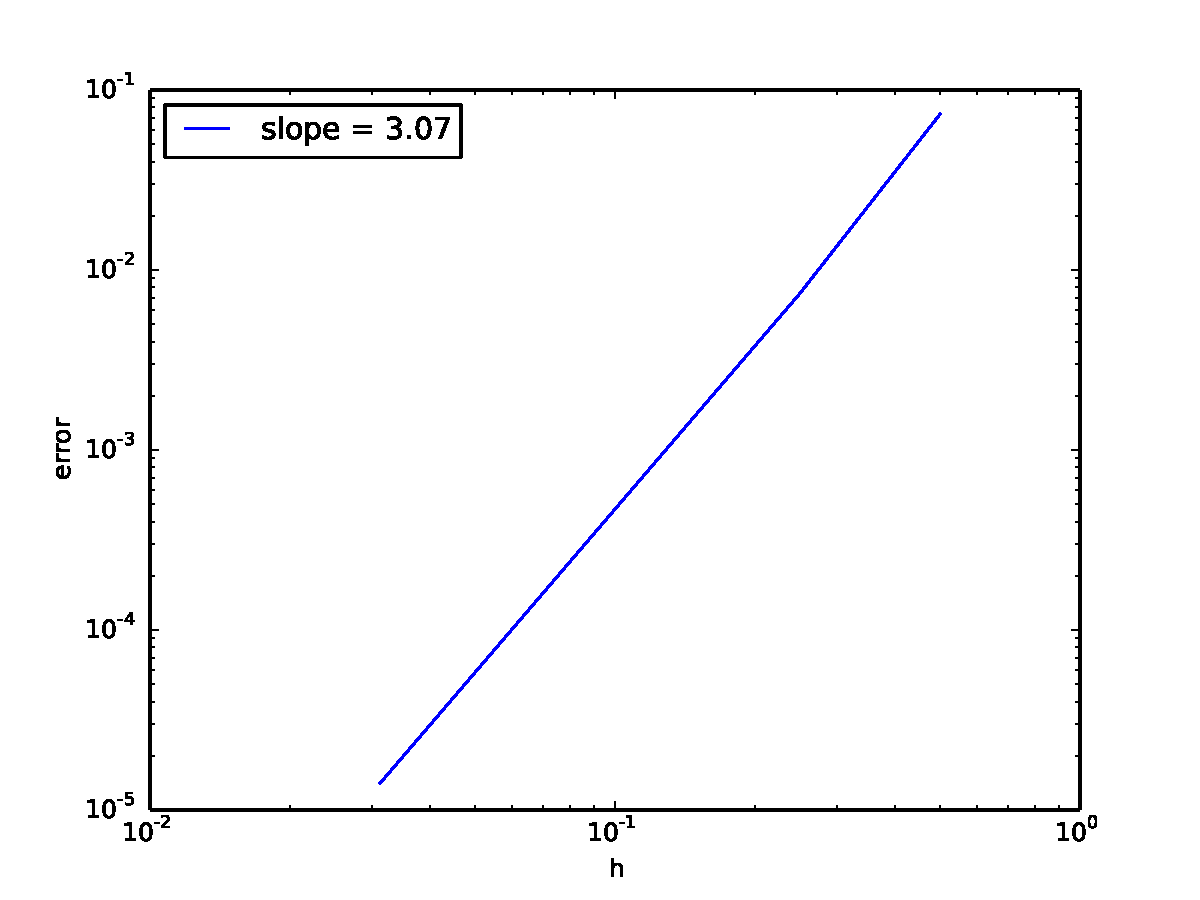
\includegraphics[width=0.7\textwidth]{SpaceTimeHeat/convergence}
	\caption{$L^2$ convergence of $u$ for the space-time heat equation}
	\label{fig:spaceTimeHeatConvergence}
\end{figure}

In order to demonstrate local space-time adaptivity we consider one more problem for the heat equation. 
On the same domain, and with the same boundary conditions as the previous example, we let the initial heat distribution be zero.
Then between $t=0.25$ and $t=0.5$ we turn on a pulse source term of one on $0.375\leq x\leq 0.625$. 
Starting from an initial mesh of $4x4$, we adaptively refine four times and obtain the results in Figure \ref{fig:spaceTimeHeatPulse}.
Notice that $\hat u$ in Figure \ref{fig:spaceTimeHeatuhat} only lives on vertical edges as was discussed earlier.
Also notice that the full mesh shown in Figure \ref{fig:spaceTimeHeatfhat} automatically adapts spatially and temporally to where features are rapidly changing. 

\begin{figure}[p]
\centering
\begin{subfigure}[t]{0.45\textwidth}
\centering
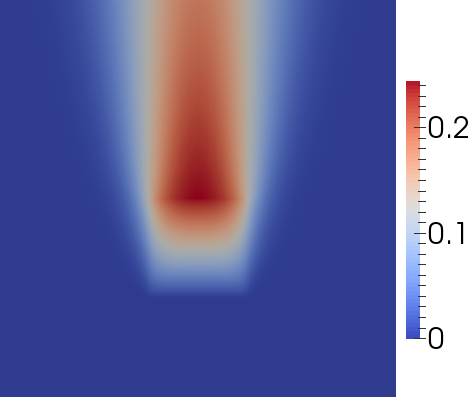
\includegraphics[width=\textwidth]{SpaceTimeHeat/PulseSource/u.png}
\caption{$u$}
\label{fig:spaceTimeHeatu}
\end{subfigure}
\begin{subfigure}[t]{0.45\textwidth}
\centering
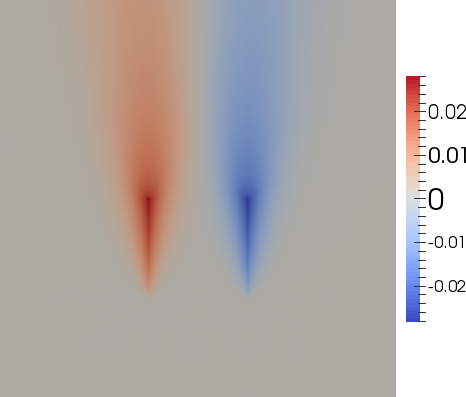
\includegraphics[width=\textwidth]{SpaceTimeHeat/PulseSource/sigma.png}
\caption{$\sigma$}
\label{fig:spaceTimeHeatsigma}
\end{subfigure}
\begin{subfigure}[t]{0.45\textwidth}
\centering
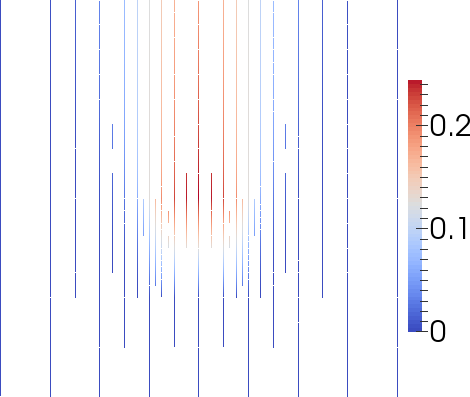
\includegraphics[width=\textwidth]{SpaceTimeHeat/PulseSource/uhat.png}
\caption{$\hat u$}
\label{fig:spaceTimeHeatuhat}
\end{subfigure}
\begin{subfigure}[t]{0.45\textwidth}
\centering
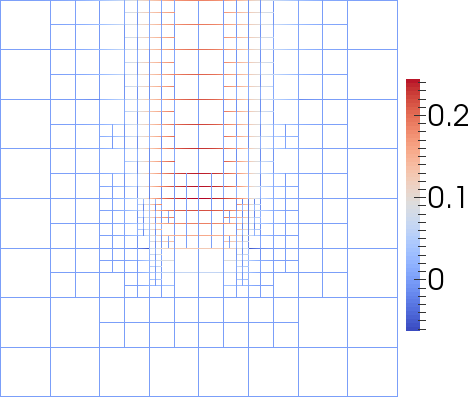
\includegraphics[width=\textwidth]{SpaceTimeHeat/PulseSource/fhat.png}
\caption{$\hat t$}
\label{fig:spaceTimeHeatfhat}
\end{subfigure}
\caption{Pulsed space-time heat problem after 4 refinements}
\label{fig:spaceTimeHeatPulse}
\end{figure}


%    /$$$$$$                       /$$$$$$                      /$$                    
%   /$$__  $$                     /$$__  $$                    |__/                    
%  | $$  \__/  /$$$$$$  /$$$$$$$ | $$  \__/ /$$   /$$  /$$$$$$$ /$$  /$$$$$$  /$$$$$$$ 
%  | $$       /$$__  $$| $$__  $$| $$$$    | $$  | $$ /$$_____/| $$ /$$__  $$| $$__  $$
%  | $$      | $$  \ $$| $$  \ $$| $$_/    | $$  | $$|  $$$$$$ | $$| $$  \ $$| $$  \ $$
%  | $$    $$| $$  | $$| $$  | $$| $$      | $$  | $$ \____  $$| $$| $$  | $$| $$  | $$
%  |  $$$$$$/|  $$$$$$/| $$  | $$| $$      |  $$$$$$/ /$$$$$$$/| $$|  $$$$$$/| $$  | $$
%   \______/  \______/ |__/  |__/|__/       \______/ |_______/ |__/ \______/ |__/  |__/
%                                                                                      
%                                                                                      
%        
\section{Convection-Diffusion}
Transient convection-diffusion is identical to the heat equation with the addition of a convective term:
\begin{equation*}
\frac{\partial u}{\partial t}+\Div(\bfbeta u)-\epsilon\Delta u=f\,.
\end{equation*}
The $d$-dimensional transient convection-diffusion equations could be viewed as a $d+1$ steady convection-diffusion problem with zero diffusion in the time direction.

\subsection{Derivation}
As a first order system in space-time, this is
\begin{equation}
\label{eq:confusionFirstOrder}
\begin{aligned}
\frac{1}{\epsilon}\bfsigma-\Grad u&=0\\
\Divxt\vecttwo{\bfbeta u-\bfsigma}{u}&=f\,.
\end{aligned}
\end{equation}
Multiplying \eqref{eq:confusionFirstOrder} by test functions, and integrating by parts over each element, we obtain the following bilinear form:
\begin{equation}
\label{eq:confusionBF}
	\begin{aligned}
		\LRp{\frac{1}{\epsilon}\bfsigma,\bftau}+\LRp{u,\Div\bftau}-\LRa{\hat u,\tau_n}&=0\\
		-\LRp{\vecttwo{\bfbeta u-\bfsigma}{u},\Gradxt v}+\LRa{\hat t,v}&=f\,,
	\end{aligned}
\end{equation}
where now $\hat t=\trace\LRp{\bfbeta u-\bfsigma}\cdot\bfn_x+\trace(u)\cdot n_t$, and $\hat u$ is as before. Our test functions, $\bftau$ and $v$ live in the same spaces as for the heat equation.

\subsection{Proof of Robustness}
Demkowicz, Heuer, and Chan\cite{DemkowiczHeuer, ChanHeuerThanhDemkowicz2012} previously completed a proof of robustness 
for the DPG method applied to steady convection-diffusion, but in this section we wish to extend those results to the transient case.


%    /$$$$$$                                                                            /$$ /$$       /$$          
%   /$$__  $$                                                                          |__/| $$      | $$          
%  | $$  \__/  /$$$$$$  /$$$$$$/$$$$   /$$$$$$   /$$$$$$   /$$$$$$   /$$$$$$$  /$$$$$$$ /$$| $$$$$$$ | $$  /$$$$$$ 
%  | $$       /$$__  $$| $$_  $$_  $$ /$$__  $$ /$$__  $$ /$$__  $$ /$$_____/ /$$_____/| $$| $$__  $$| $$ /$$__  $$
%  | $$      | $$  \ $$| $$ \ $$ \ $$| $$  \ $$| $$  \__/| $$$$$$$$|  $$$$$$ |  $$$$$$ | $$| $$  \ $$| $$| $$$$$$$$
%  | $$    $$| $$  | $$| $$ | $$ | $$| $$  | $$| $$      | $$_____/ \____  $$ \____  $$| $$| $$  | $$| $$| $$_____/
%  |  $$$$$$/|  $$$$$$/| $$ | $$ | $$| $$$$$$$/| $$      |  $$$$$$$ /$$$$$$$/ /$$$$$$$/| $$| $$$$$$$/| $$|  $$$$$$$
%   \______/  \______/ |__/ |__/ |__/| $$____/ |__/       \_______/|_______/ |_______/ |__/|_______/ |__/ \_______/
%                                    | $$                                                                          
%                                    | $$                                                                          
%                                    |__/    

\section{Nonlinear problems}

\textcolor{red}{Written by Jesse. Truman, feel free to edit it to make it match your own style}

In the context of linear problems, DPG has been successfully applied to a wide range of physical applications.  
Theoretical groundwork for DPG applied to the Poisson equation was laid in \cite{DPGPoisson}.  The time-harmonic Helmholtz equation was the focus of \cite{DPGHelmholtz, Gopalakrishnan2014} and \cite{DPG4}.  Linear elasticity and plate problems were addressed in \cite{BramwellDPG}, \cite{NiemiBramwellDemkowicz10}, and \cite{BramwellDemkowiczQiu10}, and Maxwell was addressed in \cite{DPGCloaking, WohlmuthReport}.  Linear fluid dynamics problems include convection-diffusion\cite{DPG3,DemkowiczHeuer,ChanHeuerThanhDemkowicz2012,Chan2013,EllisLC} and stationary Stokes flow\cite{DPGStokes,EllisLC}.

In the following section, we extend the idea of DPG to nonlinear problems.  In an abstract sense, we consider the nonlinear variational problem
\[
\LRa{B(u)-\ell,v}_{V^*\times V} \coloneqq \LRa{R(u),v}_{V^*\times V} = 0, \quad \forall v \in V.
\]
The linearization of this problem leads to the Newton iteration, defined by the step
\[
\LRa{J(\Delta u,u),v}_{V^*\times V} = \LRa{R(u),v}_{V^*\times V}.
\]

Moro, Peraire and Nguyen observed \cite{MoroNguyenPeraire11, MoroMastersThesis} that on a single element, the HDPG method --- referring to DPG applied to a hybridized Discontinuous Galerkin (HDG) method --- converges, while HDG on its own does not.  Moreover, HDPG required an order of magnitude less artificial diffusion to converge to a nonlinear solution of the compressible Navier-Stokes, both of which indicate strong 

In terms of comparing *competing* stabilized methods to DPG, the key here may be DPG's least-squares nature.  You might cite two references here:
- Bob, Leszek's and my paper on compressible Navier Stokes shows that even at higher Reynolds number, we converge on a coarse mesh.  I think that can be argued to be evidence of solid nonlinear stability in the pre-asymptotic regime. Burgers' equation\cite{Chan2013dpg}, incompressible Navier-Stokes\cite{NateDissertation}, and compressible Navier-Stokes\cite{JesseDissertation, Chan2013dpg}.


\subsection{Transient Compressible Navier-Stokes}
We make a large jump from convection-diffusion to the compressible Navier-Stokes equations.
The following discussion holds in any dimension, but the provided results are only for spatially 1D flows 
(at the time of this writing, our code only supported a maximum of two dimensional meshes).
The compressible Navier-Stokes equations are
\begin{align}
\frac{\partial}{\partial t}\svectthree{\rho}{\rho\bfu}{\rho e_0}
+\Div\svectthree{\rho\bfu}{\rho\bfu\otimes\bfu+p\bfI-\mathbb{D}}{\rho\bfu e_0+\bfu p+\bfq-\bfu\cdot\mathbb{D}}
%TODO: Possible error above. cfd-online seems to have T^T
=\svectthree{f_c}{\bff_m}{f_e}\,,
\end{align}
where $\rho$ is the density, $\bfu$ is the velocity, $p$ is the pressure, $\bfI$ is the identity matrix,
$\mathbb{D}$ is the deviatoric stress tensor or viscous stress, $e_0$ is the total energy, $\bfq$ is the heat flux, 
and $f_c$, $\bff_m$, and $f_e$ are the source terms for the continuity, momentum, and energy equations, respectively.
Assuming Stokes hypothesis that $\lambda=-\frac{2}{3}\mu$, 
\begin{equation*}
	\mathbb{D}=2\mu\bfS^*=2\mu\LRs{\frac{1}{2}\LRp{\Grad\bfu+\LRp{\Grad\bfu}^T}-\frac{1}{3}\Div\bfu\bfI}\,,
\end{equation*}
where $\bfS^*$ is the trace-less viscous strain rate tensor.
The heat flux is given by Fourier's law:
\begin{equation*}
	\bfq=-C_p\frac{\mu}{Pr}\Grad T\,,
\end{equation*}
where $C_p$ is the specific heat at constant pressure and $Pr$ is the laminar Prandtl number: $Pr:=\frac{C_p\mu}{\lambda}$.
We need to close these equations with an equation of state. An ideal gas assumption gives
\begin{equation*}
	\gamma:=\frac{C_p}{C_v}\,,\quad p=\rho RT\,,\quad e=C_v T\,,\quad C_p-C_v=R\,,
\end{equation*}
where $\gamma$ is the ratio of specific heats, $C_v$ is the specific heat at constant volume, $R$ is the gas constant,
$e$ is the internal energy, $T$ is the temperature,
and $\gamma$, $C_p$, $C_v$, and $R$ are constant properties of the fluid.
The total energy is defined by
\begin{equation*}
	e_0=e+\frac{1}{2}\bfu\cdot\bfu\,.
\end{equation*}

We can write our first order system of equations in space-time as follows:
\begin{subequations}
\label{eq:compressibleNSFirstOrder}
\begin{align}
	\frac{1}{\mu}\mathbb{D}-\LRp{\Grad\bfu+\LRp{\Grad\bfu}^T}+\frac{2}{3}\Div\bfu\bfI&=0\\
	\frac{Pr}{C_p\mu}\bfq+\Grad T&=0\\
	\Divxt\vecttwo{\rho\bfu}{\rho}&=f_c\\
	\Divxt\vecttwo{\rho\bfu\otimes\bfu+\rho RT\bfI-\mathbb{D}}{\rho\bfu}&=\bff_m\\
	\Divxt\vecttwo{\rho\bfu\LRp{C_v T+\frac{1}{2}\bfu\cdot\bfu}+\bfu\rho RT+\bfq-\bfu\cdot\mathbb{D}}{\rho\LRp{C_v T+\frac{1}{2}\bfu\cdot\bfu}}&=f_e\,,
\end{align}
\end{subequations}
where our solution variables are $\rho$, $\bfu$, $T$, $\mathbb{D}$, and $\bfq$.

%   /$$$$$$$                      /$$                        /$$     /$$                    
%  | $$__  $$                    |__/                       | $$    |__/                    
%  | $$  \ $$  /$$$$$$   /$$$$$$  /$$ /$$    /$$  /$$$$$$  /$$$$$$   /$$  /$$$$$$  /$$$$$$$ 
%  | $$  | $$ /$$__  $$ /$$__  $$| $$|  $$  /$$/ |____  $$|_  $$_/  | $$ /$$__  $$| $$__  $$
%  | $$  | $$| $$$$$$$$| $$  \__/| $$ \  $$/$$/   /$$$$$$$  | $$    | $$| $$  \ $$| $$  \ $$
%  | $$  | $$| $$_____/| $$      | $$  \  $$$/   /$$__  $$  | $$ /$$| $$| $$  | $$| $$  | $$
%  | $$$$$$$/|  $$$$$$$| $$      | $$   \  $/   |  $$$$$$$  |  $$$$/| $$|  $$$$$$/| $$  | $$
%  |_______/  \_______/|__/      |__/    \_/     \_______/   \___/  |__/ \______/ |__/  |__/
%                                                                                           
%                                                                                           
%              
\subsubsection{Derivation of Space-Time DPG Formulation}
We start with \eqref{eq:compressibleNSFirstOrder} and multiply by test functions $\mathbb{S}$ (symmetric tensor), $\bftau$, $v_c$, $\bfv_m$, $v_e$, 
then integrate by parts over each space-time element $K$:
\begin{subequations}
\label{eq:compressibleNSBF}
\begin{align}
	\LRp{\frac{1}{\mu}\mathbb{D},\mathbb{S}}+\LRp{2\bfu,\Div\mathbb{S}}-\LRp{\frac{2}{3}\bfu,\Grad\trace{\mathbb{S}}}
	-\LRa{\frac{4}{3}\hat\bfu,\mathbb{S}\bfn_x}&=0\\
	\LRp{\frac{Pr}{C_p\mu}\bfq,\bftau}-\LRp{T,\Div\bftau}+\LRa{\hat T,\tau_n}&=0\\
	-\LRp{\vecttwo{\rho\bfu}{\rho},\Gradxt v_c}+\LRa{\hat t_c,v_c}&=\LRp{f_c,v_c}\\
	-\LRp{\vecttwo{\rho\bfu\otimes\bfu+\rho RT\bfI-\mathbb{D}}{\rho\bfu},\Gradxt\bfv_m}+\LRa{\hat\bft_m,\bfv_m}&=\LRp{\bff_m,\bfv_m}\\
	-\LRp{\vecttwo{\rho\bfu\LRp{C_v T+\frac{1}{2}\bfu\cdot\bfu}+\bfu\rho RT+\bfq-\bfu\cdot\mathbb{D}}{\rho\LRp{C_v T+\frac{1}{2}\bfu\cdot\bfu}},\Gradxt v_e}
	+\LRa{\hat t_e,v_e}&=\LRp{f_e,v_e}\,,
\end{align}
\end{subequations}
where 
\begin{equation*}
\begin{aligned}
\hat\bfu&=\trace(\bfu)\\
\hat T&=\trace(T)\\
\hat t_c&=\trace\LRp{\rho\bfu}\cdot\bfn_x
+\trace\LRp{\rho}n_t\\
\hat\bft_m&=\trace\LRp{\rho\bfu\otimes\bfu+\rho RT\bfI-\mathbb{D}}\cdot\bfn_x
+\trace\LRp{\rho\bfu} n_t\\
\hat t_e&=\trace\LRp{\rho\bfu\LRp{C_v T+\frac{1}{2}\bfu\cdot\bfu}+\bfu\rho RT+\bfq-\bfu\cdot\mathbb{D}}\cdot\bfn_x
+\trace\LRp{\rho\LRp{C_v T+\frac{1}{2}\bfu\cdot\bfu}}n_t\,.
\end{aligned}
\end{equation*}
Note that integrating $\mathbb{S}$ against the symmetric gradient only picks up the symmetric part.
This is a much more complicated system of equations than we had for the space-time heat equation, but the situation has many similarities.
Test function $\bftau\in\HdivK$ where the divergence is taken only over spatial dimensions, $v_c,v_e\in\HOneK$, and $\bfv_m\in\HOneVecK$.
These are all familiar spaces from our work with the heat equation.
Unfortunately, $\mathbb{S}$ has some weird requirements: each $d\times d$ components must be at least in $L^2(K)$, $\Div\mathbb{S}\in\LVecK$, and
$\Grad\trace{\mathbb{S}}\in\LVecK$.
In practice, we will probably just seek each component in $\HOneK$.

%   /$$       /$$                                         /$$                       /$$     /$$                    
%  | $$      |__/                                        |__/                      | $$    |__/                    
%  | $$       /$$ /$$$$$$$   /$$$$$$   /$$$$$$   /$$$$$$  /$$ /$$$$$$$$  /$$$$$$  /$$$$$$   /$$  /$$$$$$  /$$$$$$$ 
%  | $$      | $$| $$__  $$ /$$__  $$ |____  $$ /$$__  $$| $$|____ /$$/ |____  $$|_  $$_/  | $$ /$$__  $$| $$__  $$
%  | $$      | $$| $$  \ $$| $$$$$$$$  /$$$$$$$| $$  \__/| $$   /$$$$/   /$$$$$$$  | $$    | $$| $$  \ $$| $$  \ $$
%  | $$      | $$| $$  | $$| $$_____/ /$$__  $$| $$      | $$  /$$__/   /$$__  $$  | $$ /$$| $$| $$  | $$| $$  | $$
%  | $$$$$$$$| $$| $$  | $$|  $$$$$$$|  $$$$$$$| $$      | $$ /$$$$$$$$|  $$$$$$$  |  $$$$/| $$|  $$$$$$/| $$  | $$
%  |________/|__/|__/  |__/ \_______/ \_______/|__/      |__/|________/ \_______/   \___/  |__/ \______/ |__/  |__/
%                                                                                                                  
%                                                                                                                  
%   
\paragraph{Linearization}
We follow a standard residual-Jacobian linearization procedure coupled with a Gauss-Newton solve.
Let $U=\LRc{\rho,\bfu,T,\mathbb{D},\bfq,\hat\bfu,\hat e,\hat t_c,\hat\bft_m,\hat t_e}$ be a group solution variable which we can decompose into two parts:
$U:=\tilde U+\Delta U$, where
$\tilde U = \LRc{\tilde\rho,\tilde\bfu,\tilde T,\tilde{\mathbb{D}},\bs0,\bs0,0,0,\bs0,0}$ is the previous iteration approximation, 
and $\Delta U=\LRc{\Delta\rho,\Delta\bfu,\Delta T,\Delta\mathbb{D},\bfq,\hat\bfu,\hat e,\hat t_c,\hat\bft_m,\hat t_e}$ is the update.
Note that $\tilde U$ only contains terms which participate in nonlinearities in \eqref{eq:compressibleNSBF} 
while $\Delta U$ contains the full linear terms and the updates to the nonlinear terms.
Also, we drop the $\Delta$ and $\tilde\cdot$ notation for linear terms.
Define residual $R(U)$ as the left hand side of \eqref{eq:compressibleNSBF} minus the right hand side.
Approximating $R(U)=0$ by $R(\tilde U)+R'(\tilde U)\Delta U=0$, where $R'(\tilde U)$ is the Jacobian of $R$ evaluated at $\tilde U$, we get a linear system:
\begin{equation}
	R'(\tilde U)\Delta U=-R(\tilde U)\,.
\end{equation}
This is an instance of a Gauss-Newton nonlinear solve.
We only need to define our Jacobian and residual for each component of \eqref{eq:compressibleNSBF}. 
The Jacobian of our compressible Navier-Stokes system, $R'(\tilde U)\Delta U$ is
\scriptsize
\begin{equation}
\label{eq:compressibleJacobian}
\begin{aligned}
	&\LRp{\frac{1}{\mu}\Delta\mathbb{D},\mathbb{S}}+\LRp{2\Delta\bfu,\Div\mathbb{S}}-\LRp{\frac{2}{3}\Delta\bfu,\Grad\trace{\mathbb{S}}}
	-\LRa{\frac{4}{3}\hat\bfu,\mathbb{S}\bfn_x}\\
	%
	&+\LRp{\frac{Pr}{C_p\mu}\bfq,\bftau}-\LRp{\Delta T,\Div\bftau}+\LRa{\hat T,\tau_n}\\
	%
	&-\LRp{\vecttwo{\Delta\rho\tilde\bfu+\tilde\rho\Delta\bfu}
	{\Delta\rho},\Gradxt v_c}
	+\LRa{\hat t_c,v_c}\\
	%
	&-\LRp{\vecttwo{\Delta\rho\tilde\bfu\otimes\tilde\bfu+\tilde\rho\Delta\bfu\otimes\tilde\bfu+\tilde\rho\tilde\bfu\otimes\Delta\bfu
	+\LRp{\Delta\rho R\tilde T+\tilde\rho R\Delta T}\bfI-\Delta\mathbb{D}}
	{\Delta\rho\tilde\bfu+\tilde\rho\Delta\bfu},\Gradxt\bfv_m}
	+\LRa{\hat\bft_m,\bfv_m}\\
	%
	&-\LRp{\vectthree{[C_v\Delta\rho\tilde T\tilde\bfu+C_v\tilde\rho\Delta T\tilde\bfu+C_v\tilde\rho\tilde T\Delta\bfu
	+\frac{1}{2}\LRp{\Delta\rho\tilde\bfu\cdot\tilde\bfu\tilde\bfu+\tilde\rho\Delta\bfu\cdot\tilde\bfu\tilde\bfu
	+\tilde\rho\tilde\bfu\cdot\Delta\bfu\tilde\bfu+\tilde\rho\tilde\bfu\cdot\tilde\bfu\Delta\bfu}}
	{+R\LRp{\Delta\rho\tilde T\tilde\bfu+\tilde\rho\Delta T\tilde\bfu+\tilde\rho\tilde T\Delta\bfu}
	+\bfq-\Delta\bfu\cdot\tilde{\mathbb{D}}-\tilde\bfu\cdot\Delta\mathbb{D}]}
	{C_v\Delta\rho\tilde T+C_v\tilde\rho\Delta T
	+\frac{1}{2}\LRp{\Delta\rho\tilde\bfu\cdot\tilde\bfu+\tilde\rho\Delta\bfu\cdot\tilde\bfu+\tilde\rho\tilde\bfu\cdot\Delta\bfu}},\Gradxt v_e}\\
	&+\LRa{\hat t_e,v_e}\,.
\end{aligned}
\end{equation}
\normalsize
The residual, $R(\tilde U)$, is then
\begin{equation}
\begin{aligned}
	&\LRp{\frac{1}{\mu}\tilde{\mathbb{D}},\mathbb{S}}+\LRp{2\tilde\bfu,\Div\mathbb{S}}-\LRp{\frac{2}{3}\tilde\bfu,\Grad\trace{\mathbb{S}}}\\
	&-\LRp{\tilde T,\Div\bftau}\\
	&-\LRp{\vecttwo{\tilde\rho\tilde\bfu}{\tilde\rho},\Gradxt v_c}-\LRp{f_c,v_c}\\
	&-\LRp{\vecttwo{\tilde\rho\tilde\bfu\otimes\tilde\bfu+\tilde\rho R\tilde T\bfI-\tilde{\mathbb{D}}}{\tilde\rho\tilde\bfu},
	\Gradxt\bfv_m}-\LRp{\bff_m,\bfv_m}\\
	&-\LRp{\vecttwo{\tilde\rho\tilde\bfu\LRp{C_v\tilde T+\frac{1}{2}\tilde\bfu\cdot\tilde\bfu}+\tilde\bfu\tilde\rho R\tilde T
	-\tilde\bfu\cdot\tilde{\mathbb{D}}}{\tilde\rho\LRp{C_v\tilde T+\frac{1}{2}\tilde\bfu\cdot\tilde\bfu}},
	\Gradxt v_e}-\LRp{f_e,v_e}\,.
\end{aligned}
\end{equation}

%   /$$$$$$$$                       /$$           /$$   /$$                                  
%  |__  $$__/                      | $$          | $$$ | $$                                  
%     | $$     /$$$$$$   /$$$$$$$ /$$$$$$        | $$$$| $$  /$$$$$$   /$$$$$$  /$$$$$$/$$$$ 
%     | $$    /$$__  $$ /$$_____/|_  $$_/        | $$ $$ $$ /$$__  $$ /$$__  $$| $$_  $$_  $$
%     | $$   | $$$$$$$$|  $$$$$$   | $$          | $$  $$$$| $$  \ $$| $$  \__/| $$ \ $$ \ $$
%     | $$   | $$_____/ \____  $$  | $$ /$$      | $$\  $$$| $$  | $$| $$      | $$ | $$ | $$
%     | $$   |  $$$$$$$ /$$$$$$$/  |  $$$$/      | $$ \  $$|  $$$$$$/| $$      | $$ | $$ | $$
%     |__/    \_______/|_______/    \___/        |__/  \__/ \______/ |__/      |__/ |__/ |__/
%                                                                                            
%                                                                                            
%      
\paragraph{\textcolor{red}{Test Norm}}
Usually our first choice for a DPG test norm is the graph norm which comes from upgrading the seminorm derived from the 
adjoint to a full norm.
We start by grouping terms in \eqref{eq:compressibleJacobian} by trial variable to get
\begin{equation}
\begin{aligned}
&\LRp{\Delta\mathbb{D},\frac{1}{\mu}\mathbb{S}+\Grad\bfv_m+\Grad v_e\otimes\tilde\bfu}\\
+&\LRp{\bfq,\frac{Pr}{C_p\mu}\bftau-\Grad v_e}\\
+&\left(\Delta\rho,-\tilde\bfu\cdot\Grad v_c-\frac{\partial v_c}{\partial t}
-\tilde\bfu\otimes\tilde\bfu:\Grad\bfv_m
-R\tilde T\Div\bfv_m-\tilde\bfu\cdot\frac{\partial\bfv_m}{\partial t}\right.\\
&\left.-C_v\tilde T\tilde\bfu\cdot\Grad v_e-\frac{1}{2}\tilde\bfu\cdot\tilde\bfu\tilde\bfu\cdot\Grad v_e
-R\tilde T\tilde\bfu\Grad v_e
-C_v\tilde T\frac{\partial v_e}{\partial t}-\frac{1}{2}\tilde\bfu\cdot\tilde\bfu\frac{\partial v_e}{\partial t}
\right)\\
+&\left(\Delta\bfu,2\Div\mathbb{S}-\frac{2}{3}\Grad\trace{\mathbb{S}}
-\tilde\rho\Grad v_c
-\tilde\rho\tilde\bfu\cdot\Grad\bfv_m-\tilde\rho\Grad\bfv_m\cdot\tilde\bfu
\right.\\
&\left.
-\tilde\rho\frac{\partial\bfv_m}{\partial t}
-C_v\tilde\rho\tilde T\Grad v_e
-R\tilde\rho\tilde T_\Grad v_e
+\tilde{\mathbb{D}}\cdot\Grad v_e
\right.\\
&\left.
-\frac{1}{2}\tilde\rho\tilde\bfu\cdot\tilde\bfu\Grad v_e
-\frac{1}{2}\tilde\rho\tilde\bfu\cdot\Grad v_e\tilde\bfu
-\frac{1}{2}\tilde\rho\Grad v_e\cdot\tilde\bfu\tilde\bfu
-\frac{1}{2}\tilde\rho\tilde\bfu\frac{\partial v_e}{\partial t}
-\frac{1}{2}\tilde\rho\tilde\bfu\frac{\partial v_e}{\partial t}
\right)\\
+&\left(\Delta T,-\Div\bftau
-R\tilde\rho\Div\bfv_m
-C_v\tilde\rho\tilde\bfu\Grad v_e
-R\tilde\rho\tilde\bfu\Grad v_e
-C_v\tilde\rho\frac{\partial v_e}{\partial t}
\right)\\
+&\LRp{\hat\bfu,-\frac{4}{3}\mathbb{S}\bfn_x}\\
+&\LRp{\hat T,\tau_n}\\
+&\LRp{\hat t_c,v_c}\\
+&\LRp{\hat\bft_m,\bfv_m}\\
+&\LRp{\hat t_e,v_e}\,.
\end{aligned}	
\end{equation}

Then the graph norm would be defined by
\begin{equation}
\begin{aligned}
&\norm{\frac{1}{\mu}\mathbb{S}+\Grad\bfv_m+\Grad v_e\otimes\tilde\bfu}^2\\
+&\norm{\frac{Pr}{C_p\mu}\bftau-\Grad v_e}^2\\
+&\left\|
-\tilde\bfu\cdot\Grad v_c-\frac{\partial v_c}{\partial t}-\tilde\bfu\otimes\tilde\bfu:\Grad\bfv_m
-R\tilde T\Div\bfv_m-\tilde\bfu\cdot\frac{\partial\bfv_m}{\partial t}\right.\\
&\left.-C_v\tilde T\tilde\bfu\cdot\Grad v_e-\frac{1}{2}\tilde\bfu\cdot\tilde\bfu\tilde\bfu\cdot\Grad v_e
-R\tilde T\tilde\bfu\Grad v_e
-C_v\tilde T\frac{\partial v_e}{\partial t}-\frac{1}{2}\tilde\bfu\cdot\tilde\bfu\frac{\partial v_e}{\partial t}
\right\|^2\\
+&\left\|2\Div\mathbb{S}-\frac{2}{3}\Grad\trace{\mathbb{S}}
-\tilde\rho\Grad v_c
-\tilde\rho\tilde\bfu\cdot\Grad\bfv_m-\tilde\rho\Grad\bfv_m\cdot\tilde\bfu
\right.\\
&\left.
-\tilde\rho\frac{\partial\bfv_m}{\partial t}
-C_v\tilde\rho\tilde T\Grad v_e
-R\tilde\rho\tilde T\Grad v_e
+\tilde{\mathbb{D}}\cdot\Grad v_e
\right.\\
&\left.
-\frac{1}{2}\tilde\rho\tilde\bfu\cdot\tilde\bfu\Grad v_e
-\frac{1}{2}\tilde\rho\tilde\bfu\cdot\Grad v_e\tilde\bfu
-\frac{1}{2}\tilde\rho\Grad v_e\cdot\tilde\bfu\tilde\bfu
-\frac{1}{2}\tilde\rho\tilde\bfu\frac{\partial v_e}{\partial t}
-\frac{1}{2}\tilde\rho\tilde\bfu\frac{\partial v_e}{\partial t}
\right\|^2\\
+&\left\|-\Div\bftau
-R\tilde\rho\Div\bfv_m
-C_v\tilde\rho\tilde\bfu\Grad v_e
-R\tilde\rho\tilde\bfu\Grad v_e
-C_v\tilde\rho\frac{\partial v_e}{\partial t}
\right\|^2\\
+&\alpha_c\norm{v_c}^2
+\alpha_m\norm{\bfv_m}^2
+\alpha_e\norm{v_e}^2
+\alpha_s\norm{\mathbb{S}}^2
+\alpha_f\norm{\bftau}^2
\,,
\end{aligned}
\end{equation}
where $\alpha_c$, $\alpha_m$, $\alpha_e$, $\alpha_s$, and $\alpha_f$ are scaling constants, usually one.

Unfortunately, the graph norm develops unresolvable internal boundary layers in the optimal test functions leading to a non-robust
local solve for steady convection-diffusion or Navier-Stokes,
% is known to not be robust for steady convection-diffusion or Navier-Stokes,
and we saw that non-robustness manifest when we tried to use this norm for transient simulations as well.
For steady state DPG, we developed a robust test norm for convection-diffusion and drew analogies to create 
a robust norm for Navier-Stokes.
A similar analysis for transient convection-diffusion has not been done (this is part of the proposed work), 
so we are on shakier footing developing a robust norm for transient Navier-Stokes.
Nevertheless, we can make some guesses about how to modify the test norm in order to obtain some preliminary results.
The graph norm has proven to be sufficient for simulations of pure convection. 
So an obvious first guess might be to take the graph norm on the convective quantities and decouple the viscous terms.
Indeed, this selection proved to be more robust for the test problems considered in the next section.
This modified graph norm is then:
\begin{equation}
\begin{aligned}
&\norm{\Grad\bfv_m+\Grad v_e\otimes\tilde\bfu}^2\\
+&\norm{-\Grad v_e}^2\\
+&\left\|
-\tilde\bfu\cdot\Grad v_c-\frac{\partial v_c}{\partial t}-\tilde\bfu\otimes\tilde\bfu:\Grad\bfv_m
-R\tilde T\Div\bfv_m-\tilde\bfu\cdot\frac{\partial\bfv_m}{\partial t}\right.\\
&\left.-C_v\tilde T\tilde\bfu\cdot\Grad v_e-\frac{1}{2}\tilde\bfu\cdot\tilde\bfu\tilde\bfu\cdot\Grad v_e
-R\tilde T\tilde\bfu\Grad v_e
-C_v\tilde T\frac{\partial v_e}{\partial t}-\frac{1}{2}\tilde\bfu\cdot\tilde\bfu\frac{\partial v_e}{\partial t}
\right\|^2\\
+&\left\|
-\tilde\rho\Grad v_c
-\tilde\rho\tilde\bfu\cdot\Grad\bfv_m-\tilde\rho\Grad\bfv_m\cdot\tilde\bfu
-\tilde\rho\frac{\partial\bfv_m}{\partial t}
-C_v\tilde\rho\tilde T\Grad v_e
-R\tilde\rho\tilde T\Grad v_e
+\tilde{\mathbb{D}}\cdot\Grad v_e
\right.\\
&\left.
-\frac{1}{2}\tilde\rho\tilde\bfu\cdot\tilde\bfu\Grad v_e
-\frac{1}{2}\tilde\rho\tilde\bfu\cdot\Grad v_e\tilde\bfu
-\frac{1}{2}\tilde\rho\Grad v_e\cdot\tilde\bfu\tilde\bfu
-\frac{1}{2}\tilde\rho\tilde\bfu\frac{\partial v_e}{\partial t}
-\frac{1}{2}\tilde\rho\tilde\bfu\frac{\partial v_e}{\partial t}
\right\|^2\\
+&\left\|
-R\tilde\rho\Div\bfv_m
-C_v\tilde\rho\tilde\bfu\Grad v_e
-R\tilde\rho\tilde\bfu\Grad v_e
-C_v\tilde\rho\frac{\partial v_e}{\partial t}
\right\|^2\\
+&\frac{1}{\mu}\norm{\mathbb{S}}^2
+\norm{2\Div\mathbb{S}-\frac{2}{3}\Grad\trace{\mathbb{S}}}^2
+\frac{Pr}{c_p\mu}\norm{\bftau}^2
+\norm{\Div\bftau}^2\\
+&\norm{v_c}^2
+\norm{\bfv_m}^2
+\norm{v_e}^2
\,.
\end{aligned}
\end{equation}
From a number of numerical tests, it appears that this norm is not completely robust, but it does seem to perform somewhat better
than the standard graph norm.

%   /$$   /$$                                             /$$                     /$$
%  | $$$ | $$                                            |__/                    | $$
%  | $$$$| $$ /$$   /$$ /$$$$$$/$$$$   /$$$$$$   /$$$$$$  /$$  /$$$$$$$  /$$$$$$ | $$
%  | $$ $$ $$| $$  | $$| $$_  $$_  $$ /$$__  $$ /$$__  $$| $$ /$$_____/ |____  $$| $$
%  | $$  $$$$| $$  | $$| $$ \ $$ \ $$| $$$$$$$$| $$  \__/| $$| $$        /$$$$$$$| $$
%  | $$\  $$$| $$  | $$| $$ | $$ | $$| $$_____/| $$      | $$| $$       /$$__  $$| $$
%  | $$ \  $$|  $$$$$$/| $$ | $$ | $$|  $$$$$$$| $$      | $$|  $$$$$$$|  $$$$$$$| $$
%  |__/  \__/ \______/ |__/ |__/ |__/ \_______/|__/      |__/ \_______/ \_______/|__/
%                                                                                    
%                                                                                    
% 
\subsubsection{Numerical Results}
We consider two 1D test problems as verification.
The Sod shock tube has an analytical solution derived based on an inviscid flow assumption (Euler's equations).
However, in the absence of viscosity, Euler's equations can have multiple solutions, and most numerical methods introduce a certain amount of
artificial viscosity in order to select a unique solution.
Most schemes also require the artificial viscosity to scale in some sense with mesh size so that they can effectively handle shocks.
We run our simulations without any artificial viscosity, but in order to get a well-posed problem, we do introduce a small amount of physical
viscosity: $\mu=10^{-5}$.
Essentially we are just simulating low viscosity Navier-Stokes as a stand-in for the unsolvable pure Euler.
We mentioned previously that the test norm we are using is not entirely robust, and in fact these viscosity values were on the lower end of what we
could simulate with this preliminary norm.
We solve with second order polynomial representation of field and flux variables, third order for traces, and fifth for test functions.

\paragraph{Sod Shock Tube}
The Sod shock tube problem was developed by Gary Sod in 1978\cite{Sod1978}, and has proven to be a popular problem for verification 
of compressible Navier-Stokes and Euler solvers.
It serves to verify that a numerical method can effectively handle a rarefaction wave, material discontinuity, and shock wave
all in one domain.
The Sod shock tube has an analytical solution derived based on an inviscid flow assumption (Euler's equations).
However, in the absence of viscosity, Euler's equations can have multiple solutions, and most numerical methods introduce a certain amount of
artificial viscosity in order to select a unique solution.
Most schemes also require the artificial viscosity to scale in some sense with mesh size so that they can effectively handle shocks.
We run our simulations without any artificial viscosity, but in order to get a well-posed problem, we do introduce a small amount of physical
viscosity: $\mu=10^{-5}$.
The domain of interest is a shock tube of length 1 with a material interface in the middle. The material on the left has initial conditions of 
$(\rho_L,p_L,u_L)=(1,1,0)$ while the material on the right has $(\rho_R,p_R,u_R)=(0.125,0.1,0)$; both materials have $\gamma=1.4$. 
The $t=0$ the interface between the materials is broken, 
and shock wave propagates into the right material, while a rarefaction wave moves left. The analytical solution is self-similar, but it is common to take
$t=0.2$ as a final time.
At this time the shock wave and rarefaction waves have not hit the boundaries, 
so it is sufficient to set boundary conditions corresponding to the initial conditions.
In our case, we set $\hat t_c=\hat t_m=\hat t_e=0$ on the left and right boundaries, while the fluxes are set equal to the discontinuous
initial conditions on the $t=0$ boundary. 
No boundary condition is required on the $t=0.2$ boundary since the equations are hyperbolic in time.
We solve this with one continuous time slab starting with only 4 space-time elements.
The field variables are represented with quadratics.

The results are plotted in Figure~\ref{fig:sod} for three different refinement levels: the initial coarse mesh, 7 adaptive refinements, and 14 refinements.
The coarsest mesh is obviously not sufficient to resolve the features of the flow, but it is at least somewhat representative of the exact solution.
We see significant overshoots and undershoots as we start to pick up on the shock, but these die away as we resolve to the viscous length scale.

\begin{figure}[p]
\centering
\begin{subfigure}[c]{0.3\textwidth}
\centering
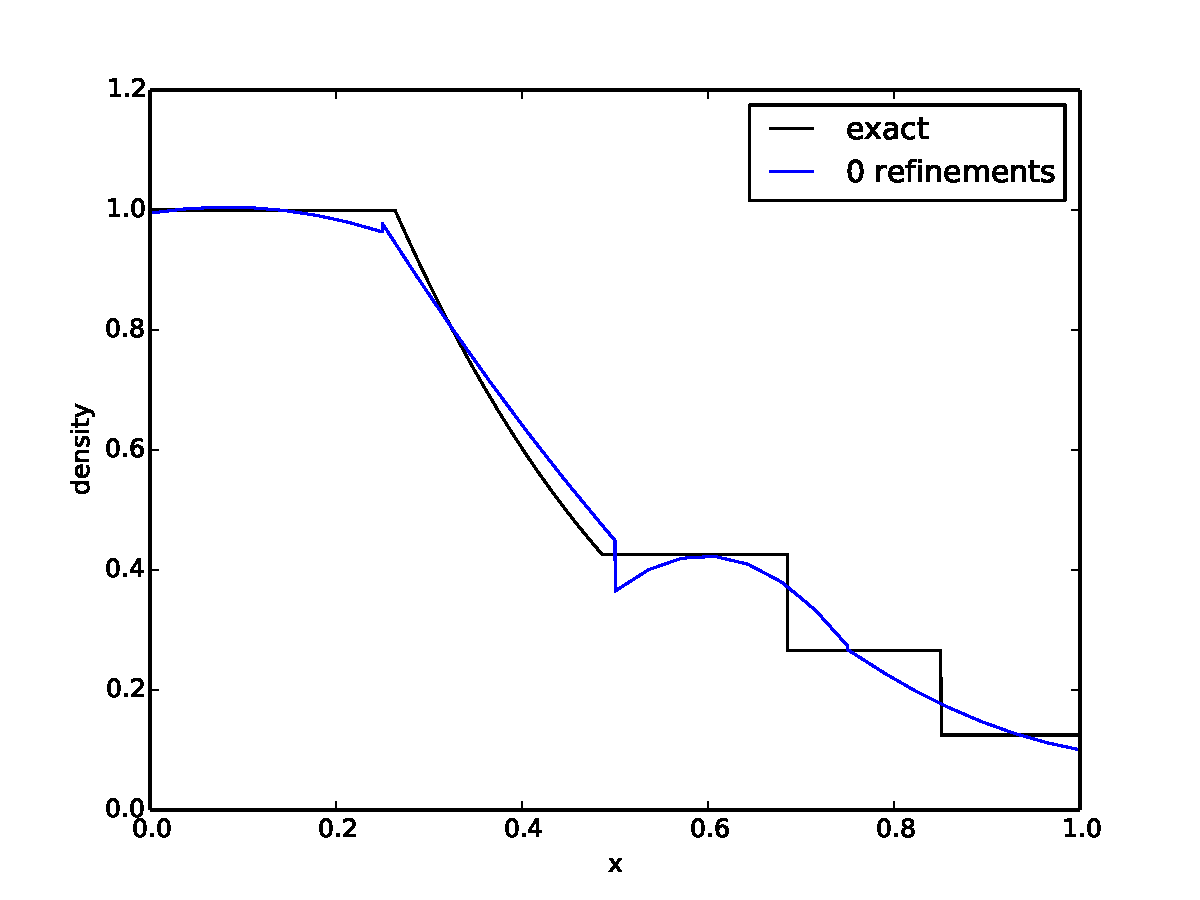
\includegraphics[width=\textwidth]{SpaceTimeCNS/Sod1e-5/den1.pdf}
\caption{Density on initial mesh}
\label{fig:sod_den0}
\end{subfigure}
\begin{subfigure}[c]{0.3\textwidth}
\centering
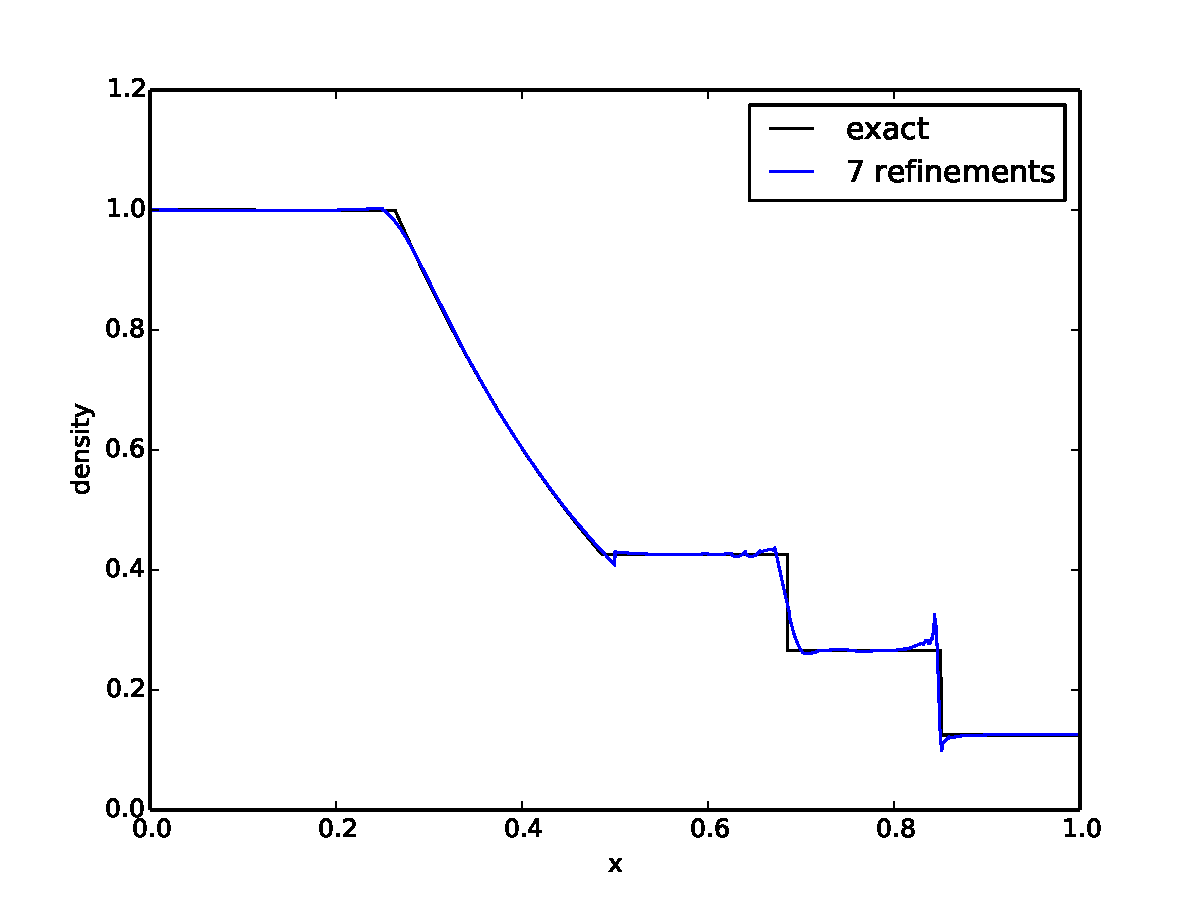
\includegraphics[width=\textwidth]{SpaceTimeCNS/Sod1e-5/den8.pdf}
\caption{After 7 refinements}
\label{fig:sod_den7}
\end{subfigure}
\begin{subfigure}[c]{0.3\textwidth}
\centering
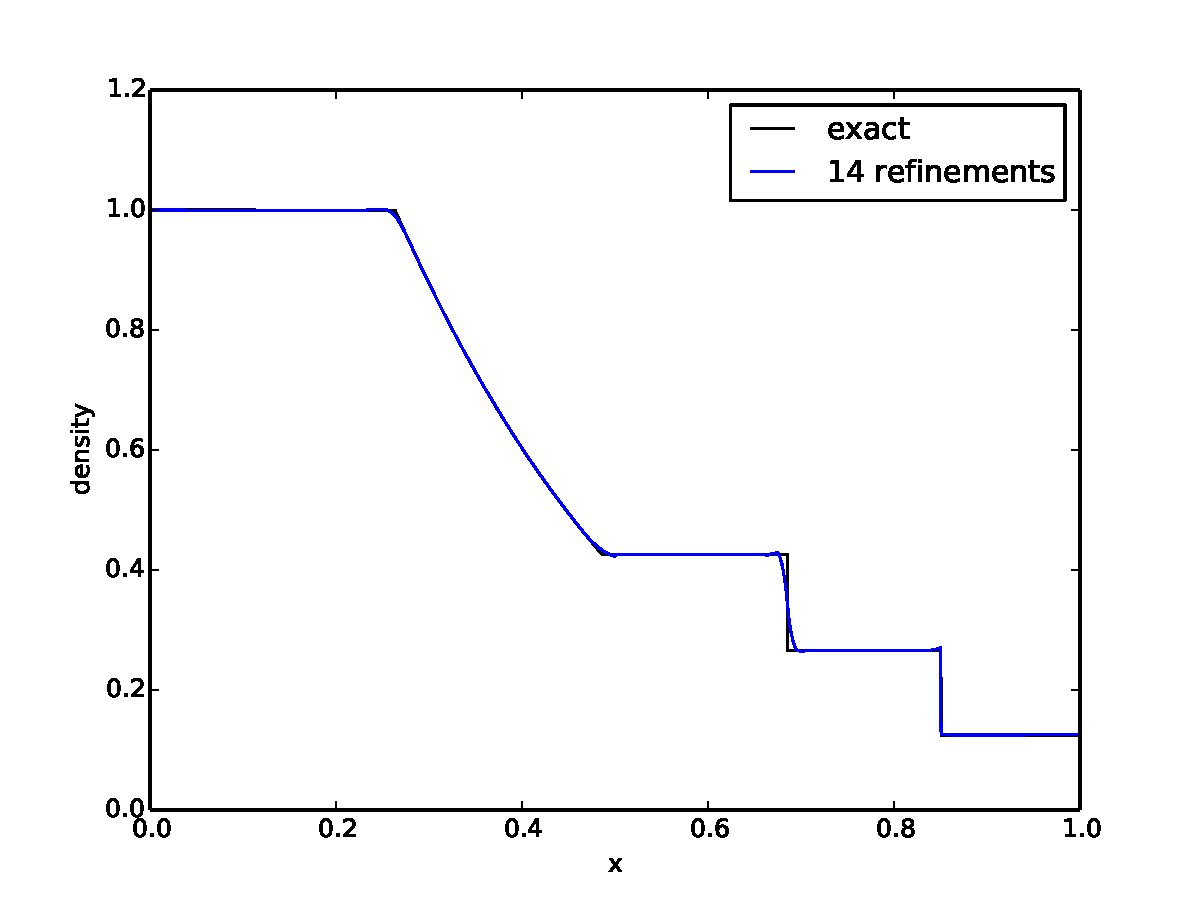
\includegraphics[width=\textwidth]{SpaceTimeCNS/Sod1e-5/den15.pdf}
\caption{After 14 refinements}
\label{fig:sod_den14}
\end{subfigure}
\begin{subfigure}[c]{0.3\textwidth}
\centering
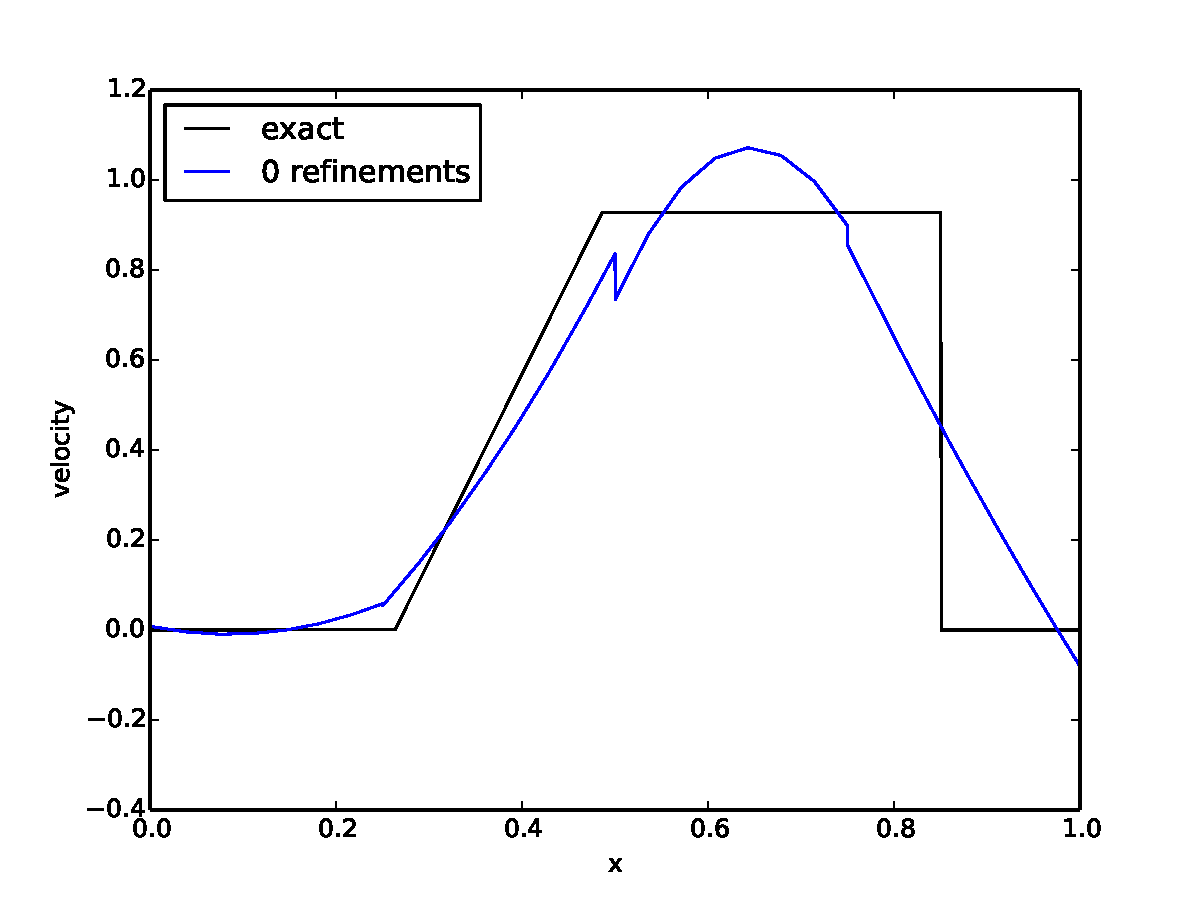
\includegraphics[width=\textwidth]{SpaceTimeCNS/Sod1e-5/vel1.pdf}
\caption{Velocity on initial mesh}
\label{fig:sod_vel0}
\end{subfigure}
\begin{subfigure}[c]{0.3\textwidth}
\centering
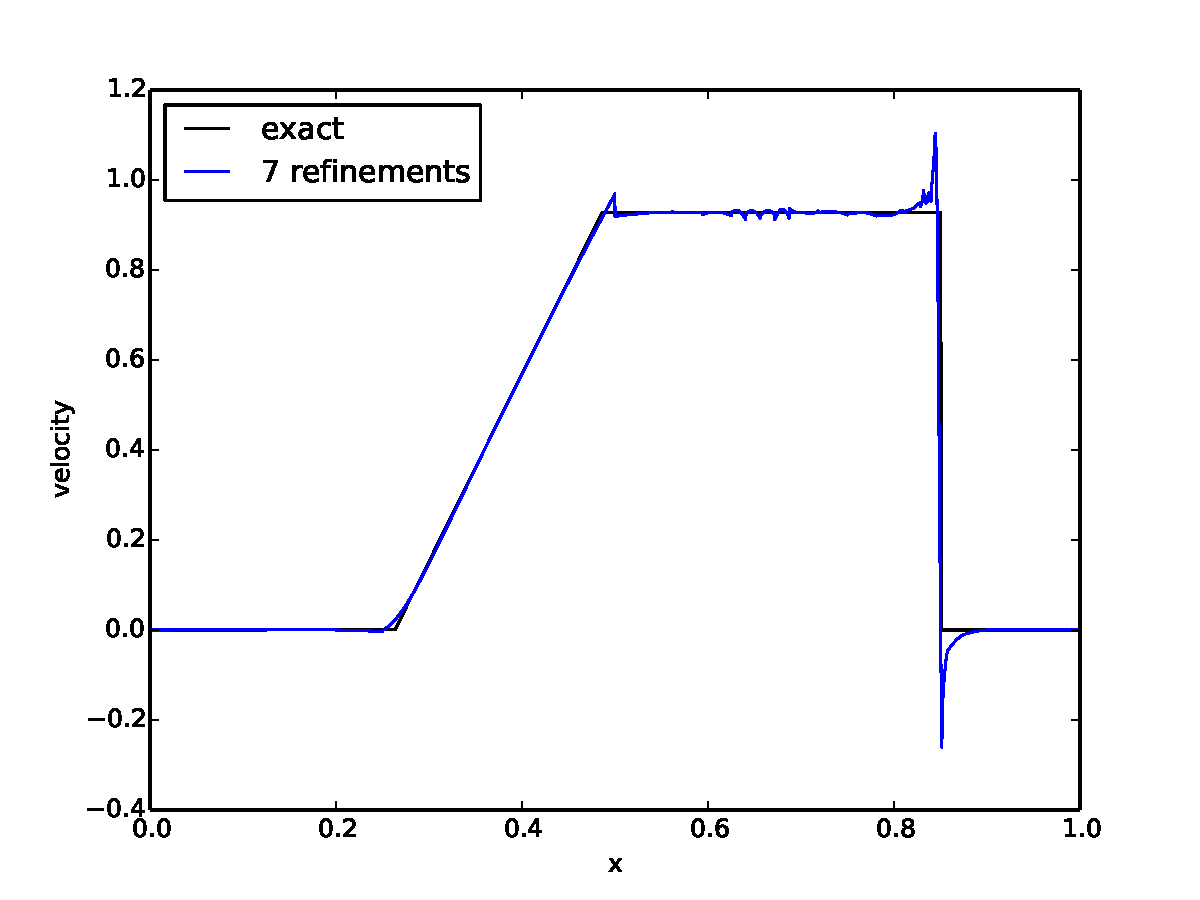
\includegraphics[width=\textwidth]{SpaceTimeCNS/Sod1e-5/vel8.pdf}
\caption{After 7 refinements}
\label{fig:sod_vel7}
\end{subfigure}
\begin{subfigure}[c]{0.3\textwidth}
\centering
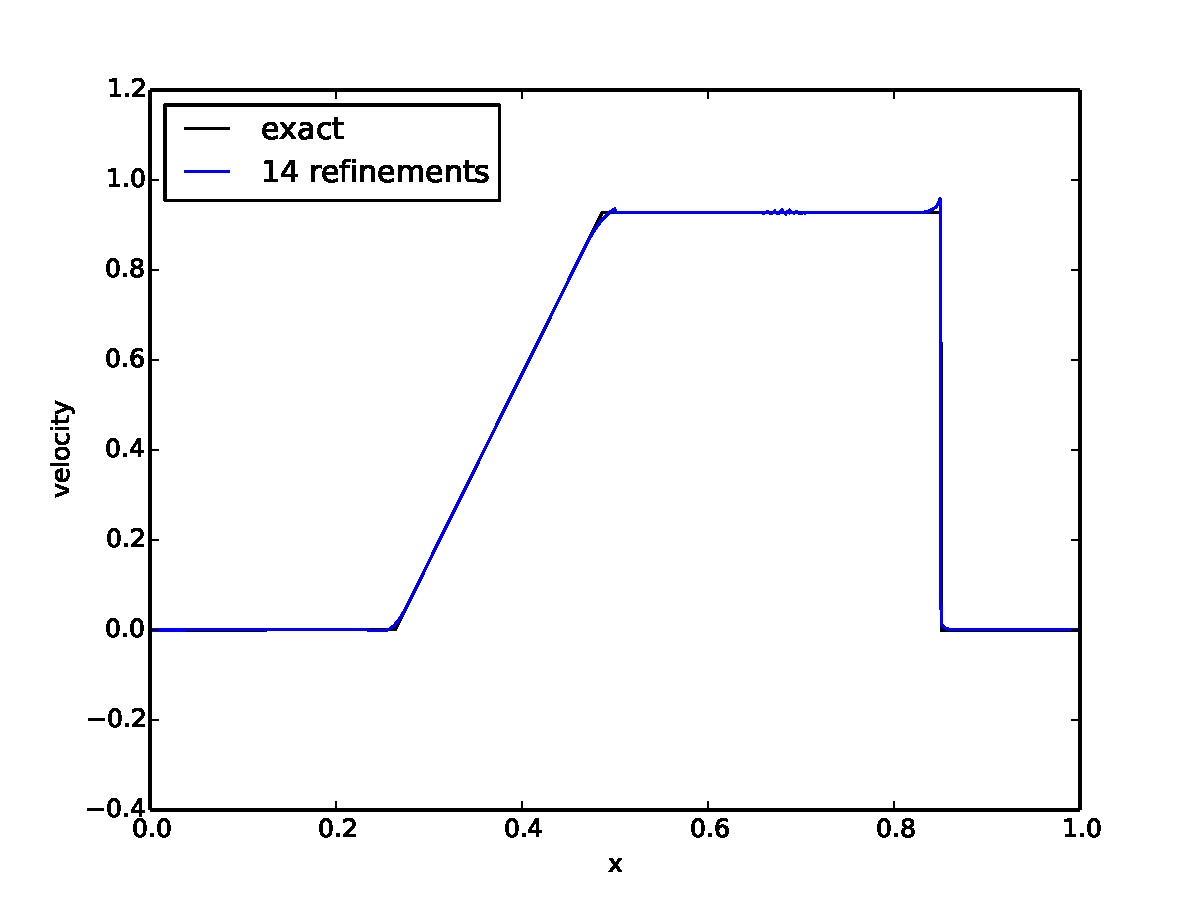
\includegraphics[width=\textwidth]{SpaceTimeCNS/Sod1e-5/vel15.pdf}
\caption{After 14 refinements}
\label{fig:sod_vel14}
\end{subfigure}
\begin{subfigure}[c]{0.3\textwidth}
\centering
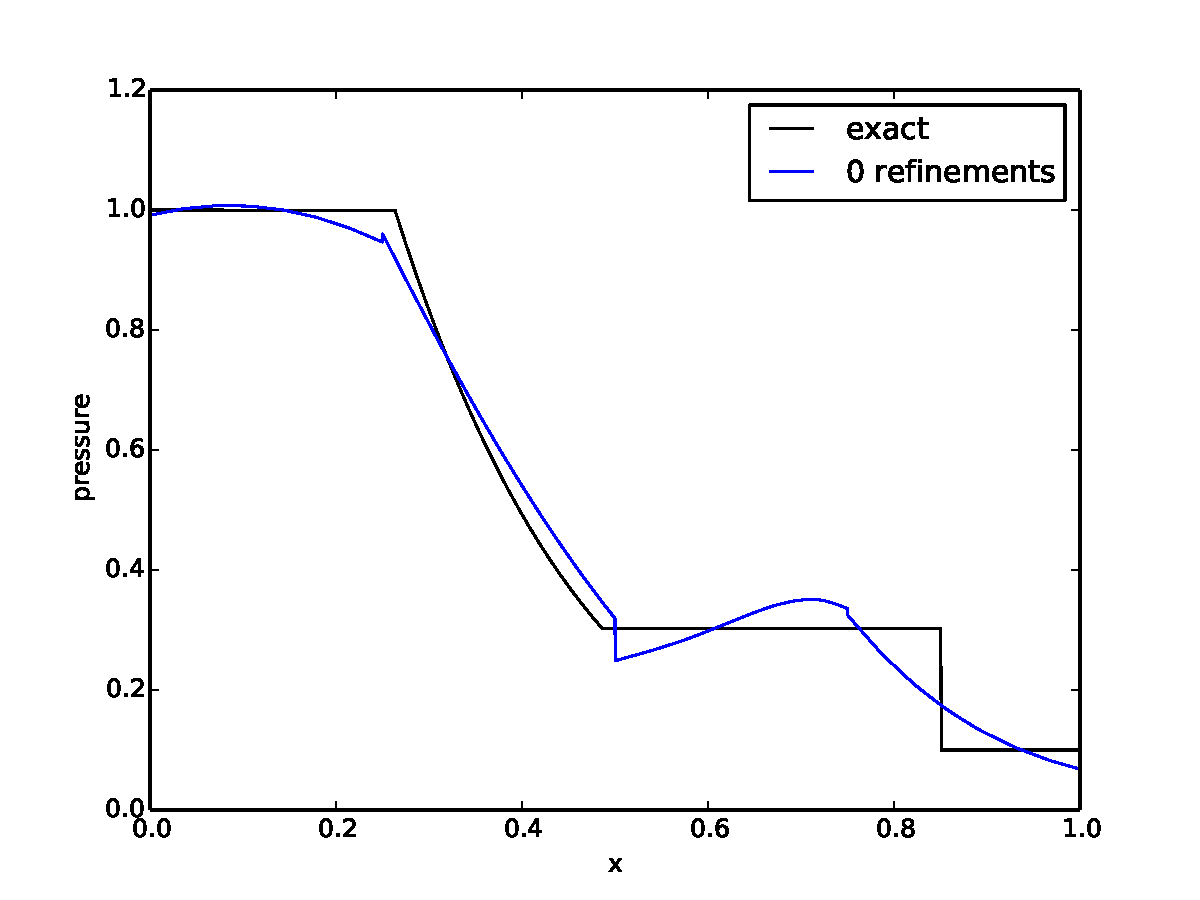
\includegraphics[width=\textwidth]{SpaceTimeCNS/Sod1e-5/pres1.pdf}
\caption{Pressure on initial mesh}
\label{fig:sod_pres0}
\end{subfigure}
\begin{subfigure}[c]{0.3\textwidth}
\centering
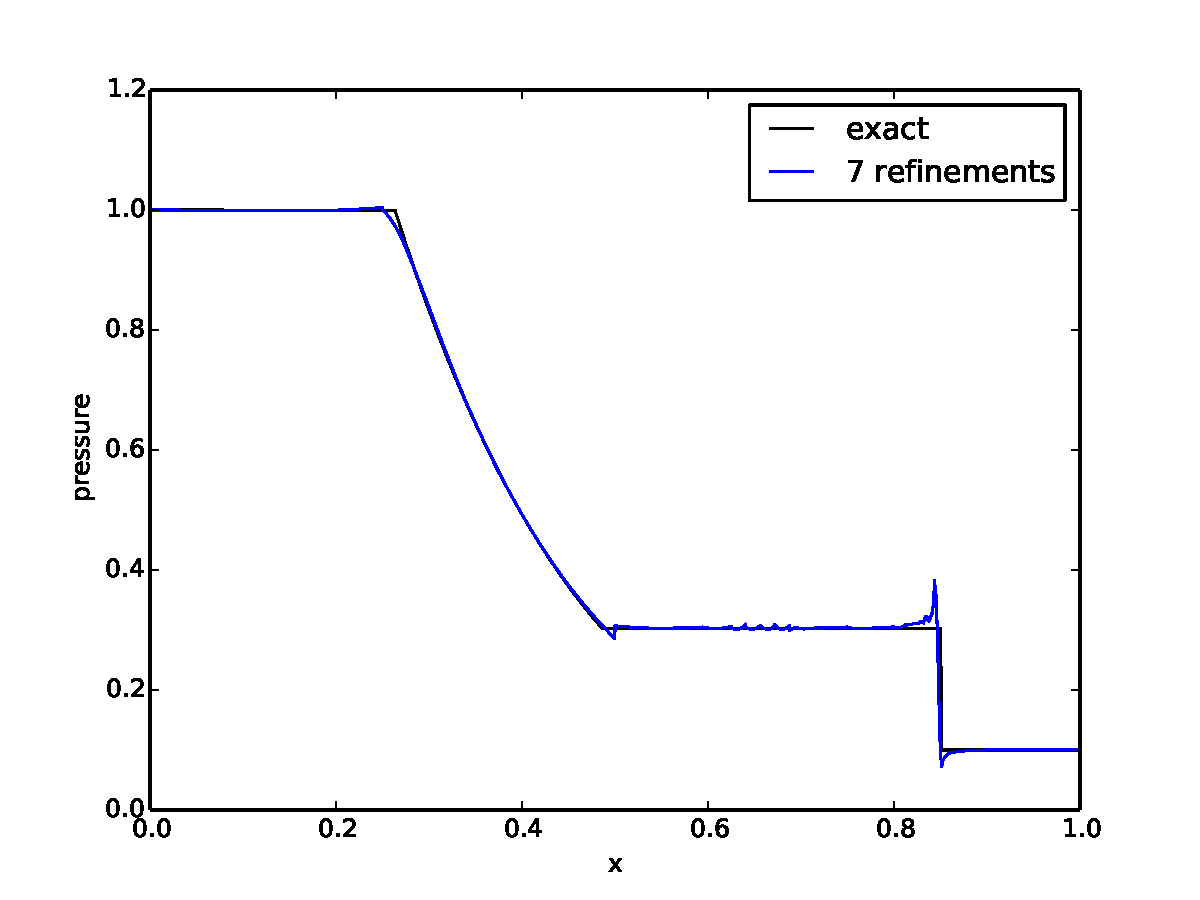
\includegraphics[width=\textwidth]{SpaceTimeCNS/Sod1e-5/pres8.pdf}
\caption{After 7 refinements}
\label{fig:sod_pres7}
\end{subfigure}
\begin{subfigure}[c]{0.3\textwidth}
\centering
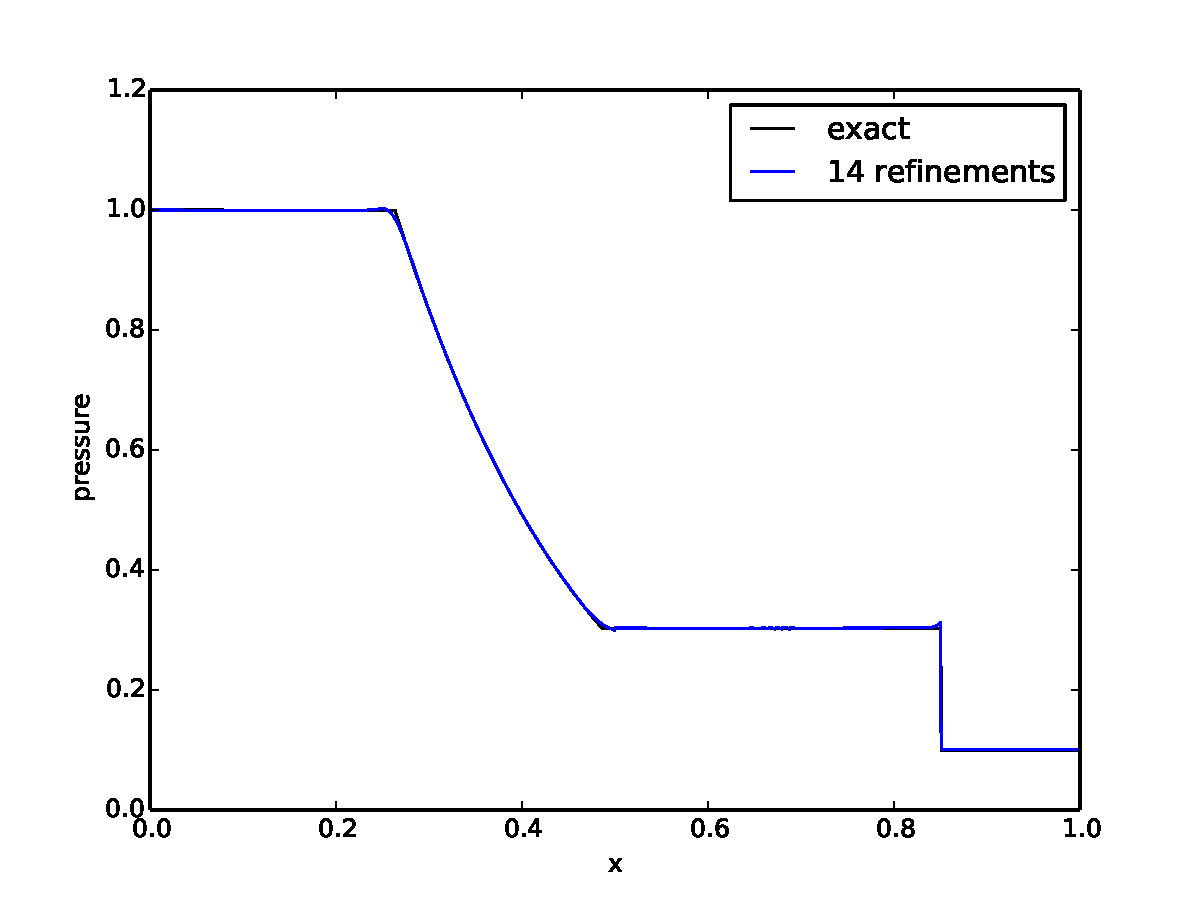
\includegraphics[width=\textwidth]{SpaceTimeCNS/Sod1e-5/pres15.pdf}
\caption{After 14 refinements}
\label{fig:sod_pres14}
\end{subfigure}
\begin{subfigure}[c]{0.45\textwidth}
\centering

\includegraphics[width=\textwidth]{SpaceTimeCNS/Sod1e-5/mesh1.png}
\caption{Density with initial mesh}
\label{fig:sod_mesh0}
\end{subfigure}
\begin{subfigure}[c]{0.45\textwidth}
\centering
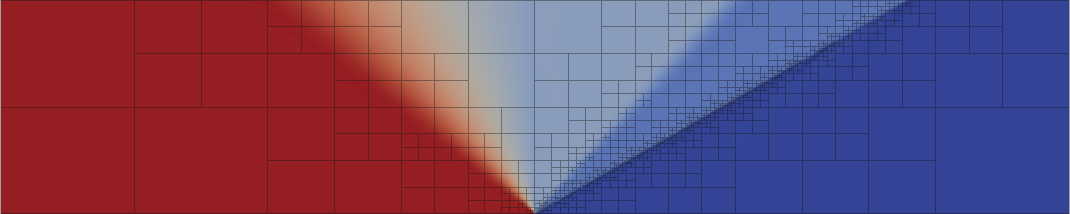
\includegraphics[width=\textwidth]{SpaceTimeCNS/Sod1e-5/mesh8.png}
\caption{Density with mesh after 7 refinements}
\label{fig:sod_mesh7}
\end{subfigure}
\begin{subfigure}[c]{0.9\textwidth}
\centering
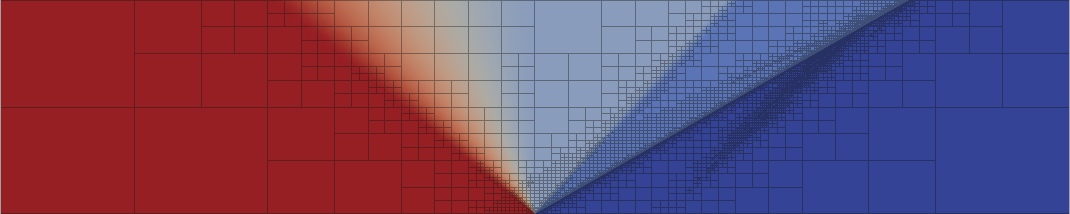
\includegraphics[width=\textwidth]{SpaceTimeCNS/Sod1e-5/mesh15.png}
\caption{Density with mesh after 14 refinements}
\label{fig:sod_mesh14}
\end{subfigure}
\caption{Sod problem with final time $t=0.2$}
\label{fig:sod}
\end{figure}

\paragraph{Noh Implosion}
The Noh implosion problem\cite{Noh1987} is another standard test for Euler solvers.
The initial conditions are of an ideal gas with $\gamma=5/3$, zero pressure, uniform initial density of 1, 
and uniform velocity toward the center of the domain.
An infinitely strong shock propagates outward at a speed of 1/3.
For 1D flow, the post shock density jumps to 4.
We run this problem to a final time of $t=1.0$.
The longer time nature of this problem recommended the use of multiple time slabs rather than a single solve like the previous problem.
We run with four time slabs of thickness 0.25 each with 4 initial space-time elements.
We run the first slab to 8 adaptive refinements and set the initial conditions on the next slab to the refined solution on the previous slab.

Each of the slabs are put together into one long time solution in Figure~\ref{fig:noh}. 
Again we plot the solution on the initial mesh, a halfway resolved mesh, and a final mesh after 8 refinement steps.
We get some very odd behavior around the shock on the middle mesh, but this goes away by the final mesh.
We see the same behavior with overshoots and undershoots that we saw with the Sod problem. 

\begin{figure}[p]
\centering
\begin{subfigure}[c]{0.3\textwidth}
\centering
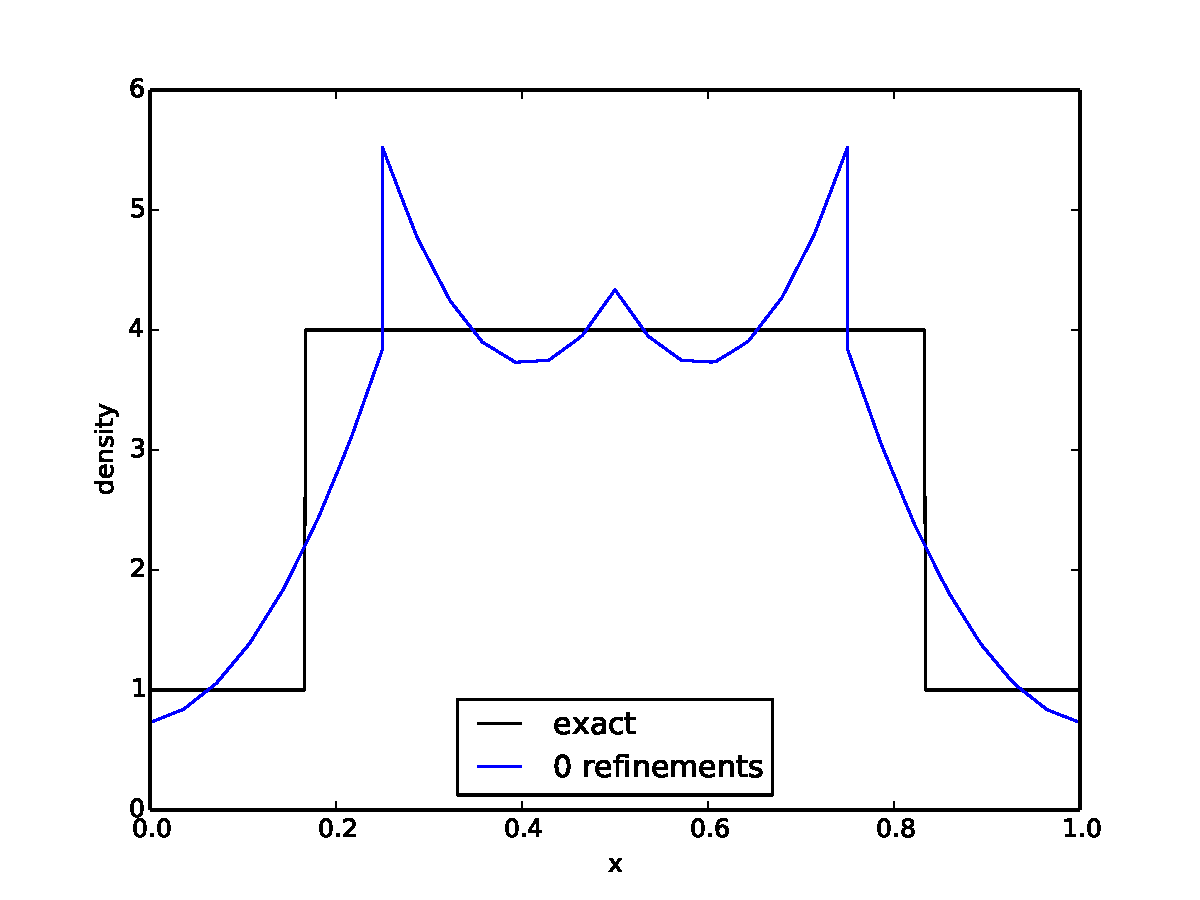
\includegraphics[width=\textwidth]{SpaceTimeCNS/Noh1e-3/den1.pdf}
\caption{Density on initial mesh}
\label{fig:noh_den0}
\end{subfigure}
\begin{subfigure}[c]{0.3\textwidth}
\centering
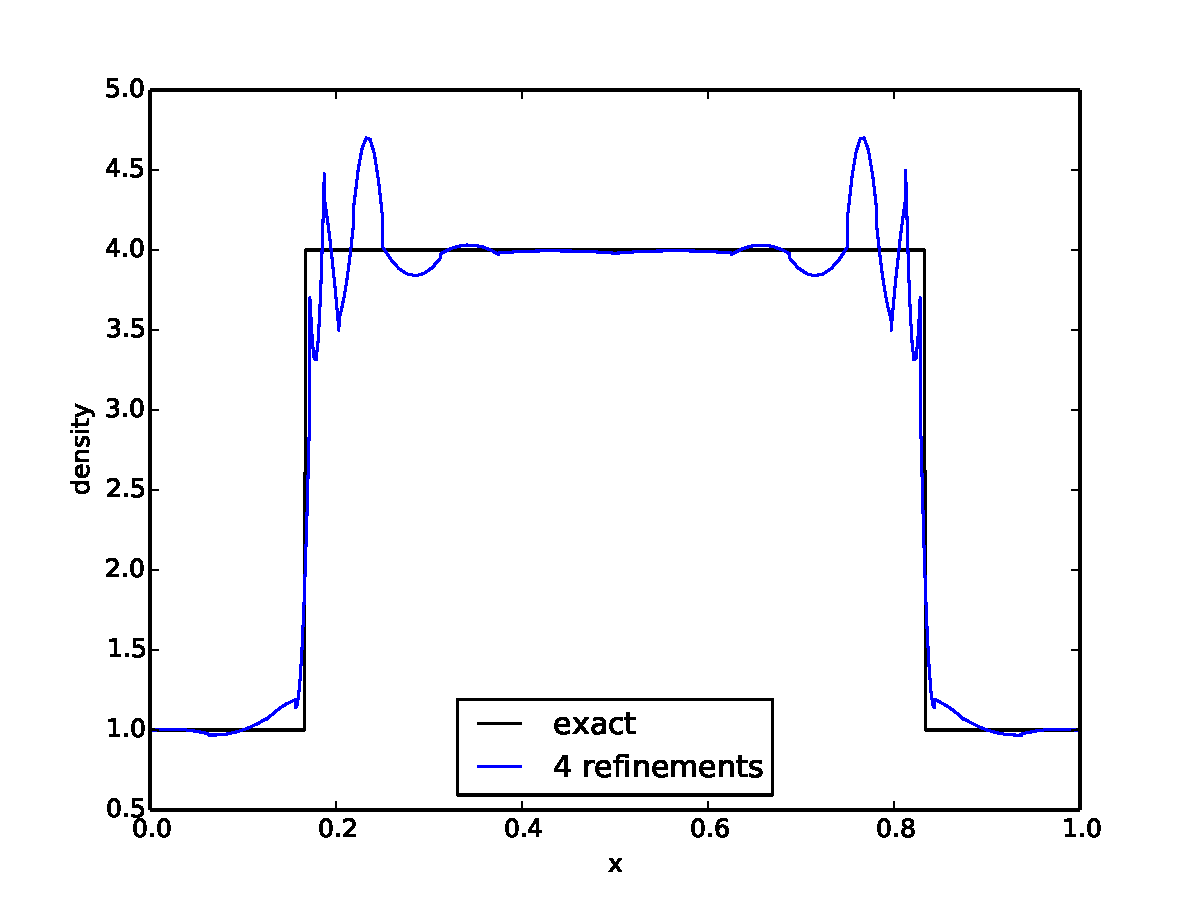
\includegraphics[width=\textwidth]{SpaceTimeCNS/Noh1e-3/den5.pdf}
\caption{After 4 refinements}
\label{fig:noh_den4}
\end{subfigure}
\begin{subfigure}[c]{0.3\textwidth}
\centering
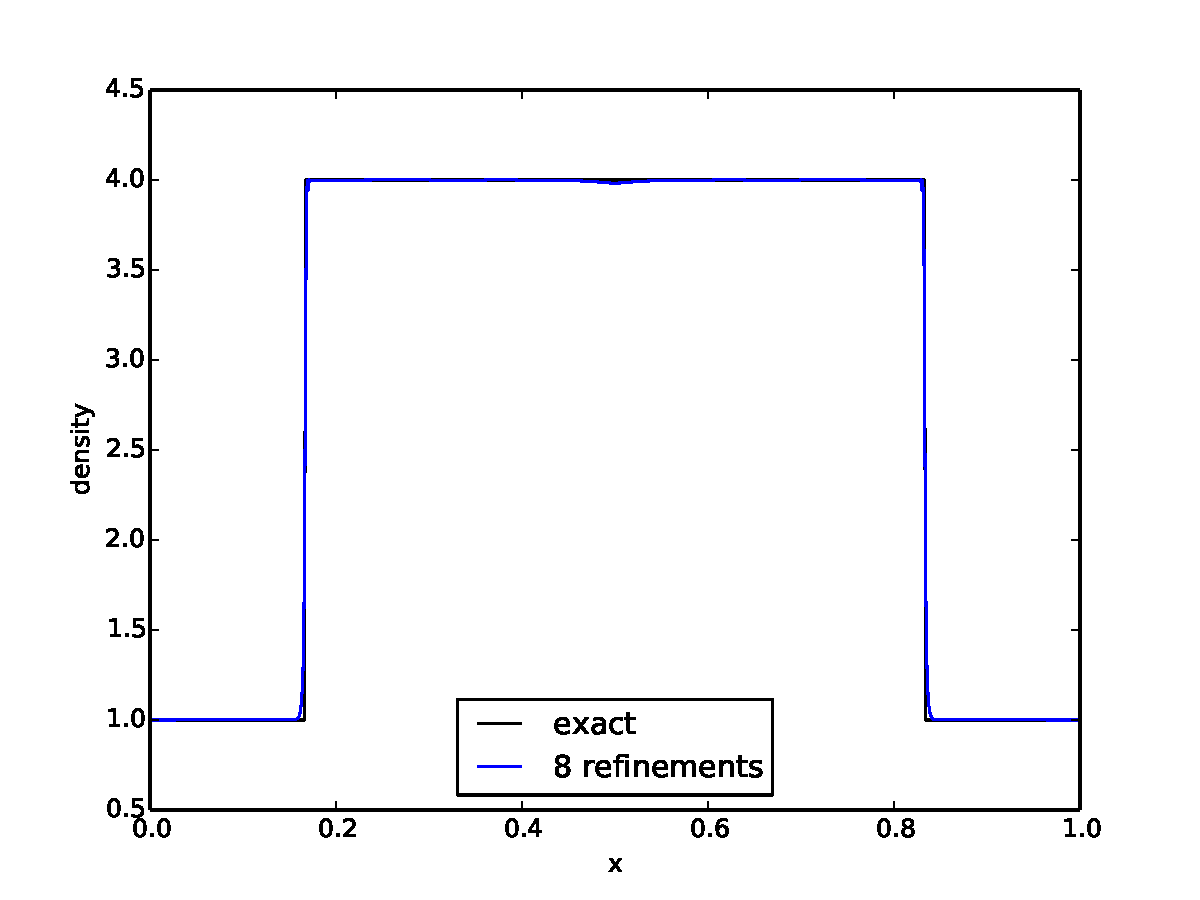
\includegraphics[width=\textwidth]{SpaceTimeCNS/Noh1e-3/den9.pdf}
\caption{After 8 refinements}
\label{fig:noh_den8}
\end{subfigure}
\begin{subfigure}[c]{0.45\textwidth}
\centering
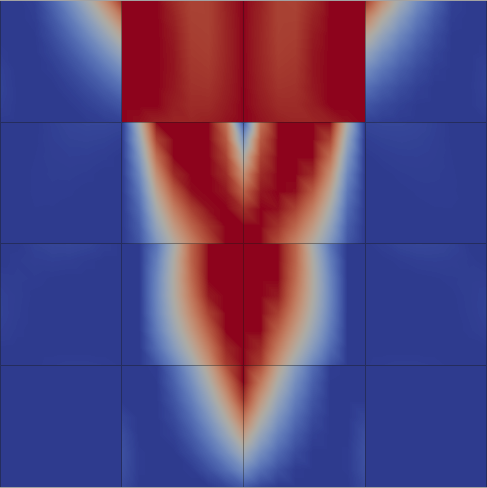
\includegraphics[width=0.65\textwidth]{SpaceTimeCNS/Noh1e-3/mesh1.png}
\caption{Density with initial mesh}
\label{fig:noh_mesh0}
\end{subfigure}
\begin{subfigure}[c]{0.45\textwidth}
\centering
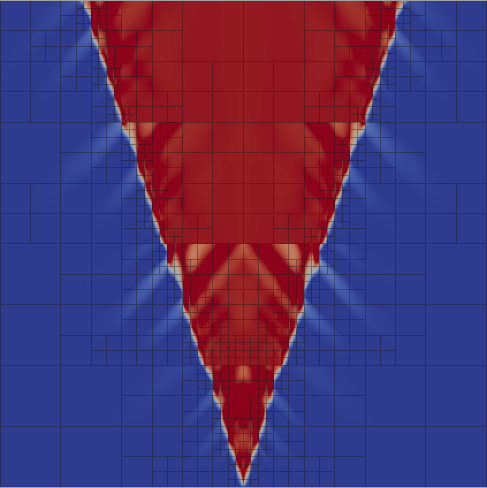
\includegraphics[width=0.65\textwidth]{SpaceTimeCNS/Noh1e-3/mesh5.png}
\caption{Density with mesh after 4 refinements}
\label{fig:noh_mesh4}
\end{subfigure}
\begin{subfigure}[c]{0.9\textwidth}
\centering
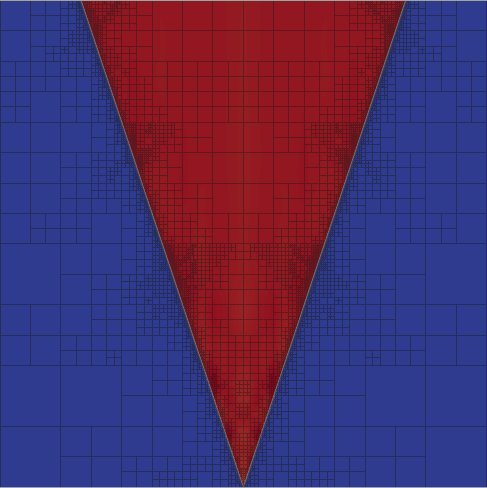
\includegraphics[width=0.65\textwidth]{SpaceTimeCNS/Noh1e-3/mesh9.png}
\caption{Density with mesh after 8 refinements}
\label{fig:noh_mesh8}
\end{subfigure}
\caption{Noh problem with final time $t=1.0$}
\label{fig:noh}
\end{figure}

\section{Conclusions and Future Work}

%% The Appendices part is started with the command \appendix;
%% appendix sections are then done as normal sections
%% \appendix

%% \section{}
%% \label{}

%% If you have bibdatabase file and want bibtex to generate the
%% bibitems, please use
%%
\bibliographystyle{elsarticle-num} 
\bibliography{../Papers}

%% else use the following coding to input the bibitems directly in the
%% TeX file.

% \begin{thebibliography}{00}

% %% \bibitem{label}
% %% Text of bibliographic item

% \bibitem{}

% \end{thebibliography}
\end{document}
\endinput
%%
%% End of file `elsarticle-template-num.tex'.
